% Original authors' source: arXiv:2501.08215v2.
% The only rendered-source change is an explicit date matching the supplied PDF.
% See README.md for provenance and build instructions.
\documentclass[a4paper,12pt]{article}
\pdfoutput=1
\usepackage[utf8]{inputenc}

\usepackage{test,graphicx,caption}
\usepackage[hyphens]{url} % to allow line break in urls

\usepackage{hyperref}
\hypersetup{colorlinks,citecolor=blue,urlcolor=magenta}
\usepackage{doi}

\usepackage[style=ext-authoryear-comp,%numeric-comp,
sorting=nyt,
dashed=false, % don't use dash for repeated author
maxcitenames=2, % maximum names to cite in text
maxbibnames=99, % maximum names to list in reference
uniquelist=false,
uniquename=false,
useprefix=true,
giveninits=true, % first name initials
natbib, % use natbib commands
date=year % year only
]{biblatex}

\AtBeginRefsection{\GenRefcontextData{sorting=ynt}}
\AtEveryCite{\localrefcontext[sorting=ynt]}

\DeclareFieldFormat{pages}{#1} % suppress pp.
\renewbibmacro{in:}{\ifentrytype{article}{}{\printtext{\bibstring{in}\intitlepunct}}} % delete In:

\DeclareFieldFormat[article,inbook,incollection,inproceedings,patent,thesis,unpublished]{titlecase:title}{\MakeSentenceCase*{#1}} % change title to sentence case

\addbibresource{localbib.bib}

\usepackage[inline,shortlabels]{enumitem}
\setlist[enumerate,1]{label=(\roman*)}

% set margin an spacing
\usepackage[margin = 1.25in]{geometry}
\usepackage{setspace}
\onehalfspacing

% custom commands

\newcommand{\AAT}[1]{{\color{magenta} AAT: #1}}
\newcommand{\KK}[1]{{\color{magenta} KK: #1}}
\renewcommand{\TH}[1]{{\color{magenta} TH: #1}}

\newcommand{\F}{\mathcal{F}}
\renewcommand{\Pr}{\operatorname{P}}

%opening
\title{Technological Innovation and Bursting Bubbles\thanks{This research was financially supported by Japan Center for Economic Research; Japan Securities Scholarship Foundation; the Joint Usage/Research Center, Institute of Economic Research, Hitotsubashi University (Grant ID: IERPK2515); JSPS KAKENHI Grant Number JP19K13660; and the Kansai University Fund for Domestic and Overseas Research Fund, 2023.}}
\author{Tomohiro Hirano\thanks{Department of Economics, Royal Holloway, University of London and the Center for Macroeconomics at the London School of Economics and the Canon Institute for
 Global Studies. Email: \href{mailto:tomohih@gmail.com}{tomohih@gmail.com}.} \and Keiichi Kishi\thanks{Faculty of Economics, Kansai University. Email: \href{mailto:kishi@kansai-u.ac.jp}{kishi@kansai-u.ac.jp}.} \and Alexis Akira Toda\thanks{Department of Economics, Emory University. Email: \href{mailto:alexis.akira.toda@emory.edu}{alexis.akira.toda@emory.edu}.}}

\numberwithin{equation}{section}
%\numberwithin{thm}{section}
%\numberwithin{lem}{section}
%\numberwithin{prop}{section}

\theoremstyle{plain}
\newtheorem{obs}{Observation}

\date{August 19, 2025}
\begin{document}
\maketitle

\begin{abstract}
We present a macro-finance model with innovation and knowledge spillover. Skilled agents engage in R\&D activities (establish firms) or work in the knowledge-intensive sector. Unskilled agents work in the traditional sector. Knowledge spillover from innovations to the two sectors is initially high and uneven (unbalanced growth), but eventually weakens and equalizes (balanced growth). A rational stock bubble (prices exceed fundamentals) necessarily emerges, even though it is expected to burst with regime switching. Despite the inevitable collapse, stock bubbles and technological innovation reinforce each other and lead to permanently higher output and wages because technologies developed during the bubble era prevail.

\medskip

\noindent
\textbf{Keywords:} balanced growth, intangible capital, stochastic bubbles, technological innovation, unbalanced growth.

\medskip

\noindent
\textbf{JEL codes:} D53, E44, G12, O30.
\end{abstract}

\section{Introduction}

Asset price bubbles are situations where asset prices ($Q$) exceed their fundamental values ($V$) defined by the expected present discounted value of future dividends ($D$). Casually looking back at the modern financial history, few would disagree that episodes such as the Mississippi and South Sea bubbles around 1720 in France and Britain, the U.S. stock market bubble in the 1920s, the Japanese stock and land bubble in the 1980s, and the U.S. dot-com bubble at the turn of the millennium qualify as bubbles. More recently, there are concerns that the AI (artificial intelligence) boom is a bubble.\footnote{\url{https://www.forbes.com/sites/johnrau/2025/01/03/is-ai-a-boom-bubble-or-con-heres-what-the-evidence-suggests/}}

Many bubbly episodes seem to be related to technological innovations. For instance, \citet[p.~1372]{Nicholas2008} states ``The 1920s [\ldots] was a period of unprecedented technological advance and intangible capital growth. [\ldots] Electricity
surpassed steam as a source of power during this decade [\ldots] Given the diffusion of the radio and the profitability of this sector, nothing was more incongruous than the collapse of the exemplar high technology stock of the 1920s--Radio Corporation
of America (RCA).'' \citet[p.~22]{Scheinkman2014} states ``Asset price bubbles tend to appear in periods of excitement about innovations. The stock market bubble of the 1920s was driven primarily by the
new technology stocks of the time, namely the automobile, aircraft, motion
picture, and radio industries, and the dotcom bubble has an obvious connection to internet technology.'' Electricity and IT (information technology) had a significant impact on production and innovation in many sectors, a characteristic that qualifies as one of the ``General Purpose Technologies (GPTs)''.\footnote{\citet{BresnahanTrajtenberg1995} characterize GPTs as displaying three fundamental features:
\begin{enumerate*}
    \item pervasiveness (they spread to a wide range of sectors),
    \item improvement (they can continuously evolve), and
    \item innovation spanning (they enhance new secondary innovations).
\end{enumerate*}}
Other booms also seem to be related to innovation, for instance Atlantic trade and insurance for the Mississippi and South Sea bubbles \citep*{FrehenGoetzmannRouwenhorst2013}, steam engine and railway network for the 1840s Railway Mania \citep[Ch.~4]{QuinnTurner2020}, and pneumatic tire for the 1890s Bicycle Mania \citep[Ch.~6]{QuinnTurner2020}.\footnote{For the cases of the 1980s Japanese stock and land bubble and the mid-2000s U.S. housing bubble, there were no clear innovations in general purpose technologies. However, there were financial innovations such as the introduction of futures, convertible bonds, securitization, and credit default swaps \citep{FostelGeanakoplos2012Tranching,HiranoToda2024JME}. See \citet{SorescuSorescuArmstrongDevoldere2018} for the connection between other technological innovations and (statistically defined) bubbles.}

Motivated by these observations, we present a macro-finance model in which technological innovation and asset price bubble reinforce each other and study the short- and long-run effects of the bubble. In our model, following the standard notion of rational bubble, a bubble means that the stock price exceeds its fundamental value defined by the expected present discounted value of future dividends ($Q>V$). Agents are rational and have common beliefs, yet they speculate on stocks. There is a unique equilibrium, and a stock market bubble necessarily emerges in this equilibrium, despite expectations that the bubble may burst at some point in the future. The bubble is caused by innovation and technological spillover, but the bubble also promotes further innovation. The bubble eventually collapses, but the positive effects on innovation prevail. This is because the new technologies and ideas that emerge during the bubble era prevail even after its collapse.

\paragraph{Toy model}
Before we present a full macro-finance model with innovation and intangible capital, we start \S\ref{sec:toy} with a toy model in an endowment economy to illustrate the key mechanism of the emergence of stochastic bubbles and identify its economic conditions and intuition. The economy is populated by overlapping generations of agents who receive endowments only when young, but they can also trade a dividend-paying asset (Lucas tree) to save for old age. To describe stochastic bubbles, we consider regime switching between two states, \ie, one ($u$) characterized by ``unbalanced growth'' where different factors of production grow at different rates, and the other ($b$) characterized by ``balanced growth'' where they grow at the same rate. State $b$ is absorbing: once the economy switches to balanced growth, it is expected to remain so indefinitely. Aggregate uncertainty arises from this regime change. In this setting, we prove the following results:
\begin{enumerate*}
    \item existence and uniqueness of equilibrium (Proposition \ref{prop:eq_toy}),
    \item impossibility of bubbles in state $b$ (Proposition \ref{prop:nobubble_toy}), and
    \item necessary and sufficient condition for the emergence of bubbles in state $u$ (Theorem \ref{thm:bubble_toy}).
\end{enumerate*}
The last condition consists of two parts, namely
\begin{enumerate*}
    \item\label{item:c1} endowments grow faster than dividends in state $u$, and
    \item\label{item:c2} upon switching to state $b$, endowments sufficiently decline.
\end{enumerate*}
Intuitively, condition \ref{item:c1} implies that as long as state $u$ persists, the asset price, pulled up by growing incomes, grows faster than dividends, resulting in an exponential rise in the price-dividend ratio. Condition \ref{item:c2} implies that the longer the bubble lasts, the greater the crash. It is the very nature of the anticipated large-scale collapse that creates the emergence of stochastic bubbles. If and only if these two conditions are simultaneously satisfied, stochastic bubbles emerge as the unique equilibrium outcome, even though they are expected to completely collapse in the future.

\paragraph{Full macro-finance model of innovation and intangible capital}
Based on the insights obtained in the toy model and motivated by the evidence of the connection between technological innovation and bubbles cited above, in \S\ref{sec:innovation}, we construct a macro-finance model of innovation and intangible capital with positive spillover to the rest of the economy. More precisely, we study a variant of the variety expansion growth model of \citet[Ch.~3]{GrossmanHelpman1991book} to analyze the relationship between knowledge spillover from knowledge-intensive sectors, such as IT and AI, to other production factors (or sectors). There are two types of agents, skilled and unskilled. Skilled agents choose to engage in R\&D activities and establish new firms or work in the knowledge-intensive sector. Unskilled agents work in the traditional sector. In \S\ref{sec:GH_bubble}, applying the results in the endowment economy, we show that stochastic stock bubbles attached to intangible capital emerge as the unique equilibrium outcome (Theorem \ref{thm:bubble_GH}). As long as state $u$ persists, where knowledge spillover is strong and unevenly spread across production factors, the economy temporarily deviates from the Balanced Growth Path (BGP) and exhibits unbalanced growth dynamics. During this phase, the knowledge-intensive sector experiences the emergence of stock bubbles with an exponential rise in the price-dividend ratio, where rising stock prices encourage the establishment of new firms and further innovations. These innovations, in turn, increase future wages, stock prices, and further innovations, creating a virtuous cycle. However, once the economy switches to state $b$, in which knowledge spillover weakens and is evenly spread across production factors, the economy returns to the BGP, the stock bubble bursts, and the price-dividend ratio stabilizes. While innovation slows down after the bubble bursts, the technologies developed during the bubble period prevail, leading to a higher level of post-bubble GDP as the bubble period lasts longer. These results are consistent with the narrative ``the relationship between bubbles and technological innovation suggests that some of these episodes may play a positive role in economic growth'' \citep[p.~40]{Scheinkman2014}. 

\paragraph{Implications for macro-theory construction}
As these models show, the dynamics with stochastic bubbles, which is characterized by unbalanced growth, can be seen as a temporary deviation from the balanced growth path in which the asset price equals the fundamental value, \ie, the expected present discounted value of future dividends. Our construction of the macro-finance model where unbalanced growth dynamics can temporarily occur provides a new perspective on the methodology of macro-theory construction because asset pricing implications markedly change. We draw an analogy to the Uzawa steady-state growth theorem, which is at the heart of macro-growth theory, and show in Proposition \ref{prop:knife-edge} that insisting  on balanced growth (and hence ruling out unbalanced growth and bubbles) requires some knife-edge restrictions on elasticities (of substitution in the production function or of knowledge spillover). As long as we impose knife-edge restrictions, it is assumed from the outset of model construction that asset prices reflect fundamentals because asset prices and dividends are assumed to grow at the same rate. What our paper shows is that even the slightest deviation from the knife-edge cases leads to markedly different implications for asset prices,\footnote{We thank Joseph Stiglitz for teaching one of the authors (Hirano) the approach ``take a standard model, change only one part, and see if it leads to markedly different economic insights''. The literature of asymmetric information pioneered by George Akerlof, Michael Spence, and Joseph Stiglitz is a notable example.} so model builders should be aware of the non-robustness introduced by knife-edge restrictions.

\paragraph{Related literature}


Our paper belongs to the so-called ``rational bubble'' literature that studies bubbles as speculation backed by nothing, which was pioneered by \citet{Samuelson1958}, \citet{Bewley1980}, \citet{Tirole1985}, \citet{ScheinkmanWeiss1986}, \citet{Kocherlakota1992}, and \citet{SantosWoodford1997}. As the literature survey of \citet{HiranoToda2024JME} shows, almost all existing research on rational bubbles focuses on so-called ``pure bubbles''---assets without dividends such as money or cryptocurrency. This is due to the ``Bubble Impossibility Theorem'' of \citet[Theorem 3.3, Corollary 3.4]{SantosWoodford1997}, which states that when the asset pays non-negligible dividends relative to the aggregate endowment, bubbles are impossible.\footnote{See \citet{Kocherlakota2008} and \citet{Werner2014} for extensions under alternative financial constraints.} However, as \citet[\S4.7]{HiranoToda2024JME} argue in detail, for describing realistic bubbles attached to dividend-paying assets like stocks, land, and housing, pure bubble models have fundamental limitations including lack of realism, equilibrium indeterminacy, and the inability to connect to the econometric literature of bubble detection. See also \citet{Barlevy2018}, who argues that pure bubble models face fundamental limitations for applications including policy and quantitative analyses. Due to the \citet{SantosWoodford1997} bubble impossibility result, there seems to be a presupposition in the macro-finance literature that the prices of dividend-paying assets should reflect fundamentals. In fact, standard macro-finance models are constructed that way.

However, the tide has turned recently and there have been a significant progress in the development of the theory of rational bubbles attached to real assets. \citet{HiranoToda2025JPE} challenge the conventional view and present a conceptually new perspective of the necessity of asset price bubbles. Within workhorse macroeconomic models without aggregate uncertainty, including overlapping generations and infinite-horizon models, they prove the existence of bubbles attached to real assets and establish the Bubble Necessity Theorem, \ie, under some conditions, the only possible equilibria are ones that feature asset price bubbles with non-negligible bubble sizes relative to the economy. In a model with aggregate uncertainty, \citet{HiranoToda2025PNAS} show that land prices exhibit recurrent stochastic fluctuations along economic development, with expansions and contractions in the size of land bubbles. In the models of \citet{HiranoToda2025JPE,HiranoToda2025PNAS}, bubbles are permanent: either there is never a bubble or there is always a bubble, with the size of bubbles expanding and shrinking. The present paper advances the direction these papers have opened up, but considers stochastic bubbles that are expected to completely collapse using the mechanism introduced by \citet{Blanchard1979} and \citet{Weil1987} in a pure bubble setting. Nevertheless, our model shows that stock bubbles inevitably emerge during the unbalanced growth regime, but they also inevitably collapse once the economy transitions to the balanced growth regime. We identify conditions under which bubbles necessarily emerge and burst. 

Finally, our paper is related to the literature on technological innovation and asset booms such as \citet{Olivier2000} and \citet{PastorVeronesi2009}. As in \citet{Olivier2000}, in our model agents establish new firms and rational bubbles are attached to dividend-paying stocks. In \citet{Olivier2000}, there exists a continuum of equilibria and the bubble is permanent. In contrast, in our model the equilibrium is unique and stock bubbles necessarily emerge,\footnote{In \citet{Olivier2000}, a critical assumption is that even though individual stocks yield the same dividend streams, all agents (including future generations) expect that stocks can be traded at different prices. In contrast, we assume that stocks with identical dividend streams are traded at the same price, as in ordinary macro-finance models.} even though they are expected to collapse completely at some point in the future. We connect the emergence and collapse of the bubble to the strength of knowledge spillover. \citet{PastorVeronesi2009} study a model of learning and technological adoption and show that the stock price can rise and fall as agents learn about and adopt the new technology, though their model is different from rational bubble.\footnote{Indeed, \citet{PastorVeronesi2009} are aware of the difference because they do not cite the literature on rational bubbles but use the term ``bubble-like'' instead.}

\section{Unique stochastic bubble in a toy model}\label{sec:toy}

To illustrate the mechanism of the emergence of stochastic bubbles in the simplest possible way, we present a toy model of an endowment economy in which an asset price bubble that is expected to collapse emerges as the unique equilibrium outcome. We then identify the economic conditions and intuition for the emergence of stochastic bubbles.  

\subsection{Model}\label{subsec:toy_model}

We consider a variant of the \citet{Lucas1978} economy. Time is indexed by $t=0,1,\dotsc$. Uncertainty is resolved according to a filtration $\set{\F_t}_{t=0}^\infty$ on a probability space $(\Omega,\F,\Pr)$. There is a single consumption good at each date, which serves as the num\'eraire. Markets are complete and all sorts of state-contingent claims (Arrow securities) in zero net supply are traded.

\paragraph{Agents and preferences}
We consider the standard two-period overlapping generations (OLG) model in which two agents (young and old) exist at each date. The OLG model is the simplest model to illustrate asset trading among heterogeneous agents that enter and exit the market. At $t=0$, there is a unit measure of initial old, who only care about their consumption. At each date $t\ge 0$, a unit measure of young agents are born, who live for two dates.

For analytical tractability, we suppose that agents have Epstein-Zin preferences with elasticity of intertemporal substitution (EIS) equal to 1.\footnote{This specification is used, for instance, in \citet[Proposition 1]{ChackoViceira2005} and \citet[Theorem 2]{TodaWalsh2020RFS}.}

\begin{asmp}\label{asmp:utility}
The utility function of an agent born at time $t$ is given by
\begin{equation}
    U(c_t^y,c_{t+1}^o)=(1-\beta)\log c_t^y+\beta\begin{cases*}
        \frac{1}{1-\gamma}\log \E_t[(c_{t+1}^o)^{1-\gamma}] & if $0<\gamma\neq 1$,\\
        \E_t[\log c_{t+1}^o] & if $\gamma=1$,
    \end{cases*}
    \label{eq:utility}
\end{equation}
Where $(c_t^y,c_{t+1}^o)$ denote consumption when young and old, $\beta\in (0,1)$ is the discount factor, $\gamma>0$ is the relative risk aversion, and $\E_t[\cdot]\coloneqq \E[\cdot|\F_t]$ denotes the expectation conditional on time $t$ information.
\end{asmp}

\paragraph{Endowments and dividends}

At date $t\ge 0$, the young are endowed with $e_t>0$ units of the good, whereas the old none.\footnote{The assumption of zero non-financial income for the old is only for analytical tractability but not essential. This assumption is adopted by \citet{Tirole1985}, \citet*{AllenBarlevyGale2025}, and \citet{HiranoToda2025PNAS}, among others.} The initial old are endowed with a unit supply of a long-lived asset (tree), which produces $D_t>0$ units of the good as dividend at date $t$.\footnote{We can think of the asset as the aggregate stock market index. Introducing multiple assets will not change the results because only the young purchase the assets and they are homogeneous, so they make the same portfolio choice, ending up demanding the market portfolio.} The sequence $\set{(e_t,D_t)}_{t=0}^\infty$ follows some stochastic process adapted to $\set{\F_t}_{t=0}^\infty$. At this point, we do not need any restriction on this stochastic process.

\paragraph{Budget constraints}

Because the young in each generation are homogeneous and demand the same portfolio, Arrow securities in zero net supply will not be traded in equilibrium. Therefore, without loss of generality we may write the budget constraints of generation $t$ as
\begin{subequations}\label{eq:budget}
\begin{align}
    &\text{Young:} & c_t^y+Q_tn_t&=e_t, \label{eq:budget_young}\\
    &\text{Old:} & c_{t+1}^o&=(Q_{t+1}+D_{t+1})n_t, \label{eq:budget_old}
\end{align}
\end{subequations}
where $Q_t>0$ is the ex-dividend asset price at time $t$ and $n_t$ is the asset holdings of generation $t$.

\paragraph{Equilibrium}

The definition of a rational expectations equilibrium is standard.

\begin{defn}\label{defn:eq_toy}
The stochastic process $\set{(Q_t,c_t^y,c_t^o,n_t)}_{t=0}^\infty$ is a \emph{rational expectations equilibrium} if
\begin{enumerate}
    \item (Utility maximization) the initial old consume $c_0^o=Q_0+D_0$; for each $t\ge 0$, $(c_t^y,n_t,c_{t+1}^o)$ maximizes the utility \eqref{eq:utility} subject to the budget constraints \eqref{eq:budget},
    \item (Commodity market clearing) for each $t$, we have $c_t^y+c_t^o=e_t+D_t$,
    \item (Asset market clearing) for each $t$, we have $n_t=1$.
\end{enumerate}
\end{defn}

Note that because the old leave the economy and hence the young are natural buyers of the asset, market clearing forces $n_t=1$. As is well known, due to unit EIS, the optimal consumption of the young is $c_t^y=(1-\beta)e_t$.\footnote{To see this, letting $c=c_t^y$, $e=e_t$, and $R=(Q_{t+1}+D_{t+1})/Q_t$ be the gross return on the asset, the optimization problem reduces to maximizing $(1-\beta)\log c+\frac{\beta}{1-\gamma}\log \left(\E[(R(e-c))^{1-\gamma}]\right)=(1-\beta)\log c+\beta \log (e-c)+\text{constant}$. Maximizing over $c$ yields $c=(1-\beta)e$.} Then, using the young's budget constraint \eqref{eq:budget_young} and the asset market clearing condition $n_t=1$, we obtain the asset price $Q_t=\beta e_t$. Therefore, we obtain the following equilibrium existence and uniqueness result.

\begin{prop}\label{prop:eq_toy}
There exists a unique rational expectations equilibrium. The asset price is $Q_t=\beta e_t$ and consumption is $(c_t^y,c_t^o)=((1-\beta)e_t,\beta e_t+D_t)$.
\end{prop}

\subsection{Fundamental value and bubble}\label{subsec:toy_bubble}

Following the standard literature of rational bubbles, we define the fundamental value of the asset by the expected present discounted value of dividends and the bubble by the difference between the asset price and its fundamental value.\footnote{See \citet{SantosWoodford1997} and \citet{HiranoToda2024JME,HiranoToda2025JPE,HiranoToda2025EJW} for more discussion.} 

Let $m_{t\to t+1}$ be the stochastic discount factor (SDF) between time $t$ and $t+1$, which we derive in \eqref{eq:SDF} below. Because the young is long in the asset, the absence of arbitrage implies
\begin{equation}
    Q_t=\E_t[m_{t\to t+1}(Q_{t+1}+D_{t+1})]. \label{eq:noarbitrage}
\end{equation}
Let
\begin{equation*}
    m_{t\to t+s}\coloneqq \prod_{j=0}^{s-1} m_{t+j\to t+j+1}
\end{equation*}
be the stochastic discount factor between time $t$ and $t+s$. Then iterating \eqref{eq:noarbitrage} from $t=0$ to $t=t-1$ and applying the law of iterated expectations, for any $t$, we obtain
\begin{equation}
    Q_0=\E_0\sum_{s=1}^t m_{0\to s} D_s+\E_0[m_{0\to t}Q_t]. \label{eq:Q_iter}
\end{equation}
Because $m_{t\to t+1}>0$ and $D_t\ge 0$, the partial sum $\E_0\sum_{s=1}^t m_{0\to s} D_s$ is increasing in $t$ and is bounded above by $Q_0$. Therefore the limit as $t\to\infty$ exists. Letting $t\to\infty$ in \eqref{eq:Q_iter} and applying the dominated convergence theorem, we obtain
\begin{equation}
    Q_0=\E_0\sum_{s=1}^\infty m_{0\to s} D_s+\lim_{t\to\infty} \E_0[m_{0\to t}Q_t]. \label{eq:Q_lim}
\end{equation}
The first term in \eqref{eq:Q_lim},
\begin{equation}
    V_0\coloneqq \E_0\sum_{s=1}^\infty m_{0\to s} D_s, \label{eq:V0}
\end{equation}
is the expected present discounted value of future dividends, which is known as the \emph{fundamental value} of the asset. The second term
\begin{equation}
    B_0\coloneqq Q_0-V_0=\lim_{t\to\infty} \E_0[m_{0\to t}Q_t]\ge 0 \label{eq:B0}
\end{equation}
is the \emph{bubble}. By definition, the asset price equals its fundamental value if and only if the no-bubble condition
\begin{equation}
    \lim_{t\to\infty} \E_0[m_{0\to t}Q_t]=0 \label{eq:nobubble}
\end{equation}
holds.\footnote{Some authors such as \citet{SantosWoodford1997}, \citet{Montrucchio2004}, and \citet{HiranoToda2025JPE} use the term ``transversality condition'' instead of ``no-bubble condition''. We use the latter to avoid the confusion between the transversality condition \emph{for asset pricing} and for \emph{optimality} (in infinite-horizon optimal control problems), which are completely different.} More generally, we have the decomposition
\begin{equation}
    Q_t=\underbrace{\E_t\sum_{s=1}^\infty m_{t\to t+s}D_{t+s}}_\text{fundamental value $V_t$}+\underbrace{\lim_{T\to\infty}\E_t[m_{t\to T}Q_T]}_\text{bubble $B_t$}. \label{eq:decompose}
\end{equation}
The economic meaning of the bubble component $B_t$ in \eqref{eq:decompose} is that it captures speculation backed by nothing, that is, agents buy the asset now for the purpose of reselling it in the future, rather than (in addition to) receiving dividends.\footnote{In fact, \citet[p.~1]{Kaldor1939} defines speculation as ``the purchase (or sale) of goods with a view to re-sale (re-purchase) at a later date''.}

When the no-bubble condition \eqref{eq:nobubble} holds, the aspect of speculation becomes negligible and asset prices are determined solely by factors that are backed in equilibrium, namely the expected future dividends. On the other hand, when $B_t>0$, asset prices contain a speculative aspect without backing and are priced above the expected present discounted value of dividends.

\subsection{Stochastic discount factor}\label{subsec:toy_SDF}

With the utility function \eqref{eq:utility} with $\gamma\neq 1$, the SDF is
\begin{equation}
    m_{t\to t+1}=\frac{\partial U/\partial c_{t+1}^o}{\partial U/\partial c_t^y}=\frac{\beta}{1-\beta}\frac{c_t^y(c_{t+1}^o)^{-\gamma}}{\E_t[(c_{t+1}^o)^{1-\gamma}]}. \label{eq:SDF}
\end{equation}
The expression \eqref{eq:SDF} is also valid for $\gamma=1$. Using the quantities in Proposition \ref{prop:eq_toy}, we may rewrite the SDF \eqref{eq:SDF} as
\begin{align}
    m_{t\to t+1}&=\frac{\beta}{1-\beta}\frac{(1-\beta)e_t (\beta e_{t+1}+D_{t+1})^{-\gamma}}{\E_t[(\beta e_{t+1}+D_{t+1})^{1-\gamma}]} \notag \\
    &=\frac{Q_t(Q_{t+1}+D_{t+1})^{-\gamma}}{\E_t[(Q_{t+1}+D_{t+1})^{1-\gamma}]}. \label{eq:SDF_Q}
\end{align}
The formula \eqref{eq:SDF_Q} turns out to be convenient, as it depends only on risk aversion and features of the asset (price and dividend).

\subsection{Temporary unbalanced growth and stochastic bubbles}

Several recent papers by some of us \citep{HiranoToda2024JME,HiranoToda2025JPE,HiranoToda2025PNAS} highlight the importance of \emph{unbalanced growth} (different sectors or factors growing at different rates) for generating asset price bubbles. However, these papers assume that the unbalanced growth dynamics is permanent. In this section, we study whether bubbles are possible when unbalanced growth occurs only temporarily, not permanently. To this end, following \citet{Weil1987}, we consider a regime-switching model with an absorbing state.

\begin{asmp}\label{asmp:states}
There are two states of the economy denoted by $u,b$. Letting $z_t\in \set{u,b}$ denote the state at time $t$, the transition probabilities are given by
\begin{align*}
    \Pr[z_{t+1}=u \mid z_t=u] &=\pi \in (0,1), \\
    \Pr[z_{t+1}=b \mid z_t=b] &=1.
\end{align*}
\end{asmp}

Assumption \ref{asmp:states} implies that state $b$ is absorbing. We further assume that, once state $b$ is reached, uncertainty is resolved and endowments and dividends grow at the same rate (balanced growth).

\begin{asmp}\label{asmp:balanced}
For any $\tau$, conditional on $z_\tau=b$, the sequence $\set{(e_t,D_t)}_{t=\tau}^\infty$ is deterministic and $e_{t+1}/e_t=D_{t+1}/D_t$ for all $t\ge \tau$.
\end{asmp}

The following proposition shows that once state $b$ is reached, there is no bubble.

\begin{prop}\label{prop:nobubble_b}
If Assumptions \ref{asmp:states}, \ref{asmp:balanced} hold, once state $b$ is reached, the asset price equals its fundamental value: $Q_t=V_t$.
\end{prop}

The intuition for Proposition \ref{prop:nobubble_b} is straightforward. By Proposition \ref{prop:eq_toy}, the asset price is proportional to endowment: $Q_t=\beta e_t$. For simplicity, assume $z_0=b$ and both endowments and dividends grow at rate $G>0$, so $e_t=e_0G^t$ and $D_t=D_0G^t$. Then the gross risk free rate equals the asset return
\begin{equation*}
    R\coloneqq \frac{Q_{t+1}+D_{t+1}}{Q_t}=G\frac{\beta e_0+D_0}{\beta e_0}>G.
\end{equation*}
Since the discount rate exceeds the growth rate of the asset, we have
\begin{equation*}
    \lim_{t\to\infty} \E_0[m_{0\to t}Q_t]=\lim_{t\to\infty}R^{-t}\beta e_0G^t=0
\end{equation*}
and the no-bubble condition \eqref{eq:nobubble} holds.

By Proposition \ref{prop:nobubble_b}, bubbles cannot arise in state $b$. Therefore, in what follows, we assume $z_0=u$. To check the no-bubble condition \eqref{eq:nobubble}, we evaluate the expectation $\E_0[m_{0\to t}Q_t]$. To simplify the calculation, let $\tau$ be the stopping time that represents the first time the economy switches to state $b$: $\tau=\min\set{t:z_t=b}$. By Assumption \ref{asmp:states}, $\tau$ is geometrically distributed with probability
\begin{equation}
    \Pr[\tau=j]=\pi^{j-1}(1-\pi) \label{eq:p_geometric}
\end{equation}
for $j=1,2,\dotsc$. Then we obtain
\begin{equation}
    \E_0[m_{0\to t}Q_t]=\sum_{j=1}^t\pi^{j-1}(1-\pi)\E_0[m_{0\to t}Q_t \mid \tau=j]+\pi^t\E_0[m_{0\to t}Q_t \mid \tau>t]. \label{eq:mQ_iter}
\end{equation}
The following proposition provides a sufficient condition for the nonexistence of bubbles.

\begin{prop}\label{prop:nobubble_toy}
Suppose Assumptions \ref{asmp:utility}--\ref{asmp:balanced} hold. Then there is no bubble if and only if
\begin{equation}
    \lim_{t\to\infty}\pi^t\E_0[m_{0\to t}Q_t \mid \tau>t]=0. \label{eq:TVC}
\end{equation}
If $(e_t,D_t)$ is known at time $t-1$ (\ie, $(e_t,D_t)$ is $\F_{t-1}$-measurable) or $\gamma=1$, then there is no bubble. 
\end{prop}

The intuition for Proposition \ref{prop:nobubble_toy} is the following. By Proposition \ref{prop:nobubble_b}, we know that there is no bubble in state $b$ and that the gross risk-free rate is higher than the growth rate of the asset price. Therefore, the conditional expectation $\E_0[m_{0\to t}Q_t \mid \tau=j]$ becomes negligible as the horizon $t$ tends to infinity. Thus, comparing the no-bubble condition \eqref{eq:nobubble} and the identity \eqref{eq:mQ_iter}, there is no bubble if and only if the last term in \eqref{eq:mQ_iter} tends to zero, or \eqref{eq:TVC} holds (the present value of resale in the far distant future is zero).

Proposition \ref{prop:nobubble_toy} implies that, to generate stochastic bubbles that are expected to collapse, endowments and dividends must not be predictable and we must move away from log utility ($\gamma=1$). Although the second point is technical, it is worth noting because the model in \citet{HiranoToda2025PNAS} generates permanent bubbles with log utility in a setting where Assumption \ref{asmp:balanced} fails (\ie, the economy never returns to balanced growth). If the economy is expected to return to balanced growth as an absorbing state (Assumption \ref{asmp:balanced}), we need stronger conditions to generate stochastic bubbles. To this end, we introduce the following assumption.

\begin{asmp}\label{asmp:conditional}
Conditional on time $t-1$ information, endowment $e_t$ and dividend $D_t$ depend only on the state $z_t\in \set{u,b}$.
\end{asmp}

Assumption \ref{asmp:conditional} implies that $(e_t,D_t)$ is stochastic conditional on time $t-1$ information (hence violating the assumption of Proposition \ref{prop:nobubble_toy}), but is a deterministic function of $z_t$. The following theorem provides a necessary and sufficient condition for the emergence of stochastic bubbles.

\begin{thm}\label{thm:bubble_toy}
Suppose Assumptions \ref{asmp:utility}--\ref{asmp:conditional} hold. For $z\in \set{u,b}$, let $(e_t^z,D_t^z)$ be the value of $(e_t,D_t)$ conditional on $z_0=\dots=z_{t-1}=u$ and $z_t=z$ and let $c_t^z\coloneqq \beta e_t^z+D_t^z$. If $z_0=u$, then there is a bubble at $t=0$ if and only if
\begin{subequations}\label{eq:finite_sum}
\begin{align}
    \sum_{t=1}^\infty D_t^u/e_t^u&<\infty, \label{eq:finite_sum1}\\
    \sum_{t=1}^\infty (c_t^b/c_t^u)^{1-\gamma}&<\infty. \label{eq:finite_sum2}
\end{align}
\end{subequations}
\end{thm}

We prove Theorem \ref{thm:bubble_toy} in the main text, as its proof is helpful to understand why the assumptions are essential.

\begin{proof}
Using the SDF \eqref{eq:SDF_Q}, we obtain
\begin{equation*}
    m_{0\to t}Q_t=\left(\prod_{s=1}^t m_{s-1\to s}\right)Q_t=Q_0\prod_{s=1}^t \frac{Q_s(Q_s+D_s)^{-\gamma}}{\E_{s-1}[(Q_s+D_s)^{1-\gamma}]}.
\end{equation*}
Let $0<Q_s^z\coloneqq \beta e_s^z=c_s^z-D_s^z$. By Assumptions \ref{asmp:states} and \ref{asmp:conditional}, conditional on $z_t=u$, it follows that
\begin{align}
    \pi^t m_{0\to t}Q_t&=Q_0\prod_{s=1}^t \frac{\pi Q_s^u(c_s^u)^{-\gamma}}{\pi (c_s^u)^{1-\gamma}+(1-\pi) (c_s^b)^{1-\gamma}} \notag \\
    &=Q_0\prod_{s=1}^t \frac{1}{1+D_s^u/Q_s^u + \frac{1-\pi}{\pi}(c_s^u/Q_s^u)(c_s^b/c_s^u)^{1-\gamma}}. \label{eq:pimQ}
\end{align}
Setting
\begin{equation}
    a_s\coloneqq D_s^u/Q_s^u+\frac{1-\pi}{\pi}(c_s^u/Q_s^u)(c_s^b/c_s^u)^{1-\gamma} \label{eq:as}
\end{equation}
and applying the inequality $\exp(a)\ge 1+a$ to the denominator of \eqref{eq:pimQ}, we obtain the lower bound
\begin{equation}
    \pi^t m_{0\to t}Q_t\ge Q_0\exp\left(-\sum_{s=1}^ta_s\right). \label{eq:pimQ_lb}
\end{equation}
Similarly, repeatedly applying the inequality $(1+a)(1+b)\ge 1+a+b$ for $a,b\ge 0$ to the denominator of \eqref{eq:pimQ}, we obtain the upper bound
\begin{equation}
    \pi^t m_{0\to t}Q_t\le Q_0\left(1+\sum_{s=1}^t a_s\right)^{-1}. \label{eq:pimQ_ub}
\end{equation}
Taking the expectations of \eqref{eq:pimQ_lb} and \eqref{eq:pimQ_ub} conditional on $\tau>t$ and letting $t\to\infty$, we obtain
\begin{equation*}
    Q_0\exp\left(-\sum_{s=1}^\infty a_s\right)\le \lim_{t\to\infty}\pi^t\E_0[m_{0\to t}Q_t\mid \tau>t]\le Q_0\left(1+\sum_{s=1}^\infty a_s\right)^{-1}.
\end{equation*}
By Proposition \ref{prop:nobubble_toy}, there is no bubble if and only if $\sum_{s=1}^\infty a_s=\infty$. Equivalently, there is a bubble if and only if $\sum_{s=1}^\infty a_s<\infty$.

If $\sum_{s=1}^\infty a_s<\infty$, because $a_s\ge D_s^u/Q_s^u$ and $Q_t=\beta e_t$, \eqref{eq:finite_sum1} must hold. Furthermore, since $a_s\to 0$, we have $D_s^u/Q_s^u\le a_s\to 0$ and $c_s^u/Q_s^u=1+D_s^u/Q_s^y\to 1$. Then \eqref{eq:as} and $\sum_{s=1}^\infty a_s<\infty$ imply \eqref{eq:finite_sum2}. Conversely, if both \eqref{eq:finite_sum1} and \eqref{eq:finite_sum2} hold, then $D_s^u/Q_s^u\to 0$ (because $Q_t=\beta e_t$) and $c_s^u/Q_s^u=1+D_s^u/Q_s^u\to 1$, so $a_s$ in \eqref{eq:as} is summable.
\end{proof}

Theorem \ref{thm:bubble_toy} can be thought of as a version of the ``Bubble Characterization Lemma'' \citep[Proposition 7]{Montrucchio2004}. The analysis in \citet{Montrucchio2004} is primarily focused on the case with aggregate uncertainty and sufficient conditions for the nonexistence of bubbles. Without aggregate uncertainty, his Proposition 7 provides a necessary and sufficient condition for the existence of bubbles, which turns out to be the same as condition \eqref{eq:finite_sum1}. Our Theorem \ref{thm:bubble_toy} extends it to the case with aggregate uncertainty, which requires more structure (Assumptions \ref{asmp:utility}--\ref{asmp:conditional}).

From the above toy model, we can draw three economic implications. 

\begin{enumerate}
    \item\label{item:imp1} First, the dynamics of asset price bubbles with an increase in the price-dividend ratio can be seen as a temporary deviation from the balanced growth path where asset prices equal the present discounted value of future dividends, \ie, the fundamentals. To see this, noting that $Q_t=\beta e_t$ and condition \eqref{eq:finite_sum1} implies $D_s^u/Q_s^u\to 0$, as long as state $u$ persists, the dividend yield converges to zero and the price-dividend ratio rises explosively.
    \item\label{item:imp2} Second, since asset prices are uniquely determined, asset price bubbles that are expected to collapse emerge as the unique equilibrium outcome. In this sense, the emergence of stochastic bubbles is a necessity, not a possibility.
    \item\label{item:imp3} Third, we can derive the economic conditions under which stochastic bubbles necessarily emerge. Assuming $\gamma<1$, these conditions are
    \begin{enumerate}
        \item\label{item:imp3a} during unbalanced growth, endowments grow faster than dividends (condition \eqref{eq:finite_sum1}), and
        \item\label{item:imp3b} when the economy switches to balanced growth, endowments sufficiently decline (condition \eqref{eq:finite_sum2}).
    \end{enumerate}
    The intuition of condition \ref{item:imp3a} is that as long as state $u$ persists, the asset price needs to grow faster than dividends. The intuition of condition \ref{item:imp3b} is that the longer the bubble lasts, the greater the crash. If and only if these two conditions are simultaneously satisfied, we will have a bubble even if unbalanced growth is temporary.
\end{enumerate}

We make two remarks. First, in the so-called ``pure bubble'' models like \citet{Samuelson1958} and \citet{Weil1987} in which the asset is intrinsically worthless, the equilibrium is indeterminate: there exist a bubbleless equilibrium, an asymptotically bubbly equilibrium, and a continuum of bubbly but asymptotically bubbleless equilibria. In this sense, bubbles are possible but not inevitable. In stark contrast, once we introduce dividends, asset price bubbles necessarily emerge under some conditions, which \citet{HiranoToda2025JPE} refer to as bubble necessity. Second, unlike the case of deterministic bubbles in which condition \ref{item:imp3a} alone is sufficient to generate bubbles without aggregate uncertainty \citep{HiranoToda2025JPE} or with aggregate uncertainty \citep{HiranoToda2025PNAS}, we also need condition \ref{item:imp3b} to generate stochastic bubbles that are expected to collapse. In other words, the very nature of the anticipated large-scale collapse is a necessary condition for the emergence of stochastic bubbles. In particular, once we consider positive dividends, a regime-switching model as in \citet{Weil1987} does not always generate stochastic bubbles because conditions \ref{item:imp3a}, \ref{item:imp3b} need not be satisfied. A natural next step is to construct a plausible economic model in which all conditions are satisfied, to which we turn next.

\section{Model of innovation and intangible capital} \label{sec:innovation}

So far, we have presented a toy model that shows the existence of stochastic bubbles in an endowment economy. In this section, we construct a macro-finance model of production economy with innovation and intangible capital and show that a stochastic stock price bubble attached to intangible capital emerges as the unique equilibrium outcome.

\subsection{Model}\label{subsec:innovation_model}

The essential structure of the model is similar to the variety expansion model of \citet[Ch.~3]{GrossmanHelpman1991book}, which builds on the monopolistic competition model of \citet{DixitStiglitz1977}. To illustrate the key mechanism of how stochastic stock bubbles emerge, we reformulate their model into an overlapping generations framework in the spirit of \S\ref{sec:toy}. An advantage of employing an OLG model is that it allows us to capture how the emergence and collapse of stock bubbles affect the generations that experienced the stock bubble and the post-bubble generation.

\paragraph{Agents}

There are two types of agents, skilled and unskilled. At each period, a mass $H>0$ continuum of skilled agents (high or human capital type) and a mass $L>0$ continuum of unskilled agents (low or labor type) are born, who live for two periods. Each individual has one unit of time to work when young and none when old. A skilled agent optimally chooses the occupation, either engaging in research and development (R\&D) activities or supplying labor for the production of knowledge-intensive intermediate goods. On the other hand, an unskilled agent inelastically supplies one unit of time to labor in the consumption good sector. As in \S\ref{sec:toy}, agents have rational expectations and lifetime utility \eqref{eq:utility}.

\paragraph{Consumption good sector}

A representative competitive firm produces the consumption good using the aggregate production function
\begin{equation}
    Y_t = F(A_{Xt}X_t,A_{Lt}L_t),    \label{eq:prod_Y}
\end{equation}
where $Y_t$ is the output of the consumption good, $X_t$ and $L_t$ are the input of knowledge-intensive good and unskilled labor, and $A_{Xt}$ and $A_{Lt}$ are their factor-augmenting productivities. We assume that the function $F(X,L)$ is neoclassical.

\begin{asmp}\label{asmp:F}
$F:\R_{++}^2\to \R_{++}$ is continuously differentiable, concave, homogeneous of degree 1, and has strictly positive partial derivatives. Furthermore, letting $g(x)\coloneqq (F_X/F_L)(x,1)$ be the marginal rate of technical substitution (where $F_X,F_L$ denote the partial derivatives with respect to $X,L$), $g$ maps $(0,\infty)$ to $(0,\infty)$.
\end{asmp}

The last condition on $g$ is a sort of Inada condition. A typical example satisfying Assumption \ref{asmp:F} is the constant elasticity of substitution (CES) specification
\begin{equation}
    F(X,L)=\begin{cases*}
        \left[ \alpha X^{1-\rho} + (1-\alpha) L^{1-\rho} \right]^{\frac{1}{1-\rho}} & if $0<\rho\neq 1$,\\
        X^\alpha L^{1-\alpha} & if $\rho=1$,
    \end{cases*} \label{eq:F_CES}
\end{equation}
where $\rho>0$ is the reciprocal of the elasticity of substitution between the two inputs and $\alpha\in (0,1)$.\footnote{The setting in \citet[Ch.~3]{GrossmanHelpman1991book} corresponds to $F(X,L)=X$ and interpreting \eqref{eq:prod_Y} as a utility function rather than a production function: see \citet[Footnote 2]{Benassy1998}. When interpreted as a utility function, households derive utility from two types of goods, $A_{Xt}X_t$ and $A_{Lt}L$.} Then straightforward algebra shows $F_X=\alpha F^\rho X^{-\rho}$ and $F_L=(1-\alpha) F^\rho L^{-\rho}$, so
\begin{equation}
    g(x)=(F_X/F_L)(x,1)=\frac{\alpha}{1-\alpha}x^{-\rho}, \label{eq:g_CES}
\end{equation}
which maps $(0,\infty)$ to $(0,\infty)$.

We take the consumption good as the num\'eraire. Taking as given the price of the knowledge-intensive good $P_t>0$ and the wage of unskilled labor $w_{Lt}>0$, the consumption good firm maximizes the profit
\begin{equation}
    Y_t-P_tX_t-w_{Lt}L_t. \label{eq:profit_Y}
\end{equation}
Because the production function \eqref{eq:prod_Y} is homogeneous of degree 1, the maximized profit is zero.

\paragraph{Knowledge-intensive good sector}

A representative competitive firm produces the knowledge-intensive good using the aggregate production function
\begin{equation}
    X_t = n_t^{1-1/\theta}\left( \int_0^{n_t} [x_t(j)]^\theta \diff j\right)^{1/\theta}, \label{eq:prod_X}
\end{equation}
where $X_t$ is the output of the knowledge-intensive good, $n_t$ is the measure of intermediate good variety existing at time $t$, $x_t(j)$ is the input of the intermediate good of variety $j$, and $\theta \in (0,1)$ is an elasticity parameter. (The elasticity of substitution satisfies $\varepsilon\coloneqq 1/(1-\theta)>1$.) The coefficient $n_t^{1-1/\theta}$ in \eqref{eq:prod_X} is a scaling factor to disentangle market power and taste for variety (or productivity): see \citet{Benassy1996,Benassy1998}. For simplicity, we refer to $n_t$ as knowledge. As we describe below, $n_t$ endogenously grows as a result of innovation (R\&D). Taking as given the price of the knowledge-intensive good $P_t>0$ and the prices of intermediate goods $\set{p_t(j)}_{j\in [0,n_t]}$, the knowledge-intensive good firm maximizes the profit
\begin{equation}
    P_tX_t-\int_0^{n_t} p_t(j)x_t(j)\diff j. \label{eq:profit_X}
\end{equation}
Again because the production function \eqref{eq:prod_X} is homogeneous of degree 1, the maximized profit is zero.

\paragraph{Intermediate good sector}

Each intermediate good $j$ is produced by a single monopolistically competitive firm using skilled labor as input. One unit of skilled labor produces one unit of the intermediate good. Thus, taking the wage of skilled labor $w_{Ht}>0$ as given, firm $j$ chooses the price $p_t(j)$ and quantity $x_t(j)$ to maximize the profit
\begin{equation}
    d_t(j)=(p_t(j)-w_{Ht})x_t(j), \label{eq:profit_j}
\end{equation}
where firm $j$ understands that $x_t(j)$ equals the demand obtained by maximizing \eqref{eq:profit_X}. The profit $d_t(j)$ in \eqref{eq:profit_j} is distributed as dividends to the shareholders of firm $j$.

\paragraph{R\&D sector}

New intermediate good varieties are created through R\&D. Letting $n_t$ be the knowledge at time $t$, a unit of skilled labor engaging in R\&D at time $t$ creates $an_t$ units of new intermediate good varieties, where $a>0$ is a productivity parameter. The term $n_t$ in the R\&D production function $an_t$ captures knowledge spillover from existing innovations to new ones.\footnote{As is well known in the endogenous growth literature such as \citet{Romer1990}, this linearity assumption of knowledge spillover is necessary to generate endogenous growth. Our setup is equivalent to Equation (3.21) of \citet[p.~58]{GrossmanHelpman1991book}, where our $a$ and $n_t$ correspond to their $1/a$ and $K_n$.}

The newly invented varieties are fully protected by patents indefinitely. A new firm $j$ issues a unit of stock and sells in an initial public offering (IPO) at price $q_t(j)$. Firm $j$'s stock is a claim to the dividend stream (monopoly profit) \eqref{eq:profit_j}. The IPO revenue accrues to the founding skilled agent. The stock price $q_t(j)$ can also be interpreted as the price of an idea or patent, \ie, intangible capital.\footnote{Instead of patent protection for good production, we may keep the ideas as trade secrets. The analysis remains the same if we assume that a trade secret can fully protect the idea. Therefore, we may interpret $q_t(j)$ as intangible capital.}

\subsection{Equilibrium}

Loosely speaking, given the initial knowledge $n_0$ and the stochastic process of productivities $\set{(A_{Xt},A_{Lt})}_{t=0}^\infty$, an equilibrium is a situation in which agents optimally choose occupation and maximize utility subject to budget constraints, firms maximize profits, and all markets (consumption good, knowledge-intensive good, intermediate good, skilled labor, unskilled labor, and stocks) clear. We characterize the equilibrium.

\paragraph{Firms}

The first-order conditions for the profit maximization problem \eqref{eq:profit_Y} are
\begin{subequations}
\begin{align}
    P_t&=F_X(A_{Xt}X_t,A_{Lt}L)A_{Xt}. \label{eq:Pt} \\
    w_{Lt}&=F_L(A_{Xt}X_t,A_{Lt}L)A_{Lt}, \label{eq:wLt}
\end{align}
\end{subequations}
where we have imposed the unskilled labor market clearing condition $L_t=L$. The first-order condition for the profit maximization problem \eqref{eq:profit_X} with respect to intermediate good $j$ is
\begin{equation*}
    p_t(j)=P_tn_t^{1-1/\theta}\left( \int_0^{n_t} [x_t(j)]^\theta \diff j\right)^{1/\theta-1}x_t(j)^{\theta-1}=P_t(X_t/n_t)^{1-\theta}x_t(j)^{\theta-1},
\end{equation*}
where $X_t$ is the knowledge-intensive good \eqref{eq:prod_X}. Solving this expression for $x_t(j)$, we obtain the demand for the intermediate good $j$
\begin{equation}
    x_t(j)=(X_t/n_t)(p_t(j)/P_t)^{-\frac{1}{1-\theta}} \label{eq:xtj}
\end{equation}
as a function of the intermediate good price $p_t(j)$. Substituting the demand \eqref{eq:xtj} into the profit \eqref{eq:profit_j} and maximizing over $p_t(j)$, by elementary calculus we obtain the monopoly price
\begin{equation}
    p_t(j)=\frac{w_{Ht}}{\theta}, \label{eq:ptj}
\end{equation}
which is common across all intermediate good firms. As is well known in the literature of monopolistic competition \citep{DixitStiglitz1977}, the price is marked above the marginal cost $w_{Ht}$ by the factor $1/\theta>1$. Because the price $p_t(j)$ is common, so is the quantity $x_t(j)\eqqcolon x_t$ in \eqref{eq:xtj}. Using \eqref{eq:prod_X}, we obtain
\begin{equation}
    X_t=n_t^{1-1/\theta}(n_tx_t^\theta)^{1/\theta}=n_tx_t. \label{eq:Xt}
\end{equation}
Substituting \eqref{eq:Xt} into \eqref{eq:xtj} and \eqref{eq:profit_j}, we obtain the price of the knowledge-intensive good $P_t=p_t(j)=w_{Ht}/\theta$ and dividend
\begin{equation}
    d_t(j)=\frac{1-\theta}{\theta}w_{Ht}x_t. \label{eq:dtj}
\end{equation}

\paragraph{Agents}

By \eqref{eq:dtj}, all stocks pay the same dividend $D_t\coloneqq d_t(j)$. We consider an equilibrium in which all stocks trade at the common price $Q_t\coloneqq q_t(j)$.

A type $H$ (skilled) agent has the option of either working in the knowledge-intensive intermediate good sector and earning wage $w_{Ht}$ or engaging in R\&D, creating $an_t$ new firms, and earning the IPO profit $an_tQ_t$. Thus, assuming innovation occurs, the indifference condition is
\begin{equation}
    an_tQ_t=w_{Ht}. \label{eq:indifference}
\end{equation}
Using \eqref{eq:Xt}--\eqref{eq:indifference}, the dividend yield is
\begin{equation}
    \frac{D_t}{Q_t}=\frac{1-\theta}{\theta}w_{Ht}x_t/\frac{w_{Ht}}{an_t}=a\frac{1-\theta}{\theta}X_t. \label{eq:divyield1}
\end{equation}

Let $n_{it}$ be the demand for stocks by an agent of type $i\in \set{H,L}$ and $(c_{it}^y,c_{i,t+1}^o)$ be consumption when young and old. The budget constraints are
\begin{subequations}\label{eq:budget_GH}
\begin{align}
    &\text{Young:} & c_{it}^y+Q_tn_{it}&=w_{it}, \label{eq:budget_GH_young}\\
    &\text{Old:} & c_{i,t+1}^o&=(Q_{t+1}+D_{t+1})n_{it}. \label{eq:budget_GH_old}
\end{align}
\end{subequations}
As in \S\ref{sec:toy}, because optimal consumption is $c_{it}^y=(1-\beta)w_{it}$ and savings is $\beta w_{it}$, we have
\begin{subequations}\label{eq:nHLt}
\begin{align}
    n_{Ht}&=\beta w_{Ht}/Q_t=\beta an_t, \label{eq:nHt}\\
    n_{Lt}&=\beta w_{Lt}/Q_t=(w_{Lt}/w_{Ht})\beta an_t. \label{eq:nLt}
\end{align}
\end{subequations}

\paragraph{Equilibrium}

We now derive the equilibrium condition. Let $\phi_t\in (0,1]$ be the fraction of skilled agents working in the knowledge-intensive intermediate good sector. Since the demand for skilled labor is $n_tx_t$ and the mass of skilled agents is $H$, the market clearing condition for skilled labor is
\begin{equation}
    X_t=n_tx_t=\phi_t H. \label{eq:laborH}
\end{equation}
By definition, the mass of skilled agents engaging in R\&D is $(1-\phi_t)H$. Hence the number of stocks outstanding at the end of period $t$ is the number of initially traded stocks $n_t$ plus new issuance $an_t(1-\phi_t)H$, so
\begin{equation}
    n_{t+1}=(1+a(1-\phi_t)H)n_t. \label{eq:n_dyn}
\end{equation}
The stock market clearing condition at the end of period $t$ is
\begin{equation}
    \underbrace{n_{t+1}}_\text{supply}=\underbrace{Hn_{Ht}+Ln_{Lt}}_\text{demand}. \label{eq:n_clear}
\end{equation}

Under the maintained assumptions, we can prove the existence and uniqueness of equilibrium.

\begin{prop}\label{prop:eq_GH}
Suppose Assumptions \ref{asmp:utility}, \ref{asmp:F} hold. Then there exists a unique rational expectations equilibrium. If
\begin{equation}
    \frac{1}{aH}<\beta+\beta\left[\theta\frac{A_{Xt}H}{A_{Lt}L}g\left(\frac{A_{Xt}H}{A_{Lt}L}\right)\right]^{-1}, \label{eq:phi_cond}
\end{equation}
the fraction $\phi_t$ of skilled agents working in the intermediate good sector satisfies
\begin{equation}
    \frac{1}{aH}=\phi_t-1+\beta+\beta\left[\theta\frac{A_{Xt}H}{A_{Lt}L}g\left(\frac{A_{Xt}H}{A_{Lt}L}\phi_t\right)\right]^{-1}. \label{eq:eqcond1}
\end{equation}
If \eqref{eq:phi_cond} does not hold, then $\phi_t=1$ and there is no innovation. In either case, $\phi_t$ depends on $t$ only through the relative productivity $A_{Xt}/A_{Lt}$. Furthermore, the equilibrium prices are determined by
\begin{subequations}\label{eq:eqprice}
\begin{align}
    &\text{Knowledge-intensive good price:} & P_t&=p_t(j)=F_XA_{Xt}, \label{eq:eqprice_P}\\
    &\text{Skilled wage:} & w_{Ht}&=\theta F_XA_{Xt}, \label{eq:eqprice_wH}\\
    &\text{Unskilled wage:} & w_{Lt}&=F_LA_{Lt}, \label{eq:eqprice_wL}\\
    &\text{Stock price:} & Q_t&=\frac{w_{Ht}}{an_t}=\frac{\theta}{an_t}F_XA_{Xt}, \label{eq:eqprice_Q}
\end{align}
where $F_X,F_L$ are evaluated at $(A_{Xt}H\phi_t,A_{Lt}L)$.
\end{subequations}
\end{prop}

\section{Emergence of stochastic stock bubbles}\label{sec:GH_bubble}

In this section, we specialize the general model of \S\ref{sec:innovation} to study the emergence of stochastic stock bubbles.

\subsection{Assumptions}

Following the setting in \S\ref{sec:toy}, agents have Epstein-Zin utility (Assumption \ref{asmp:utility}). There are two aggregate states denoted by $z\in \set{u,b}$, where $u,b$ correspond to unbalanced growth and balanced growth, with $b$ absorbing (Assumption \ref{asmp:states}). The aggregate production function takes the CES form \eqref{eq:F_CES}. Regarding the factor-augmenting productivities, we impose the following assumption.

\begin{asmp}\label{asmp:AZ}
There exist constants $A_X,A_L>0$ and $\xi_u,\xi_b,\lambda_u,\lambda_b\ge 0$ such that
\begin{equation}
    (A_{Xt},A_{Lt})=(A_Xn_t^{\xi_{z_t}},A_Ln_t^{\lambda_{z_t}}). \label{eq:AXLt}
\end{equation}
Furthermore, the following conditions hold:
\begin{subequations}
\begin{align}
    \psi&\coloneqq (\xi_u-\lambda_u)(\rho-1)>0, \label{eq:xi} \\
    \lambda_u&>\lambda_b=\xi_b. \label{eq:alphazeta}
\end{align}
\end{subequations}
\end{asmp}

Several remarks are in order. The parametric form of productivities \eqref{eq:AXLt} implies that there is a positive spillover from knowledge $n_t$ to production factors, which is a common assumption in endogenous growth models \citep{Frankel1962,Romer1986}. The condition \eqref{eq:xi} implies that, in particular, $\lambda_u\neq \xi_u$ and $\rho\neq 1$. The condition $\lambda_u\neq \xi_u$ implies that when innovation generates new technologies, its spillover effects are unevenly spread across the two production factors, and hence their productivity growth rates are different. We refer to this situation as \emph{unbalanced growth}. Recalling that the elasticity of substitution between unskilled labor and the knowledge-intensive good is $1/\rho$ and empirical estimates of the elasticity of substitution in the aggregate production function is often less than 1 \citep{OberfieldRaval2021,GechertHavranekIrsovaKolcunova2022}, condition \eqref{eq:xi} holds if $\xi_u>\lambda_u$ and $\rho>1$, \ie, knowledge spillover is stronger in the knowledge-intensive good sector. The condition $\lambda_u>\lambda_b\ge 0$ implies that there is knowledge spillover from existing innovations to the productivity of unskilled labor $L$. Furthermore, the spillover is stronger in state $u$. This assumption is natural if we consider how innovations such as personal digital assistants (\ie, tablets), the Internet, and artificial intelligence improved the productivity of ordinary workers by making routine work more efficient. Finally, the condition $\lambda_b=\xi_b$ implies that once the state $b$ is reached, the spillover effects of innovation decrease and spread evenly throughout the economy. This condition ensures the existence of a balanced growth path (BGP) along which aggregate consumption, investment in R\&D, and dividends are constant fractions of GDP. Note that $\lambda_b=\xi_b$ is a knife-edge condition, but as noted in the introduction, any growth model with BGP is knife-edge theory.

Under the maintained assumptions, the equilibrium condition \eqref{eq:eqcond1} reduces to
\begin{equation}
    \frac{1}{aH}=\phi_t-1+\beta+\frac{\beta(1-\alpha)}{\theta\alpha}\left(\frac{A_XH}{A_LL}\right)^{\rho-1}n_t^{(\xi_{z_t}-\lambda_{z_t})(\rho-1)}\phi_t^\rho. \label{eq:eqcond2}
\end{equation}
To sustain innovation, we impose the following initial condition.

\begin{asmp}\label{asmp:n0}
Initial knowledge $n_0$ satisfies
\begin{equation}
    \frac{1}{aH}<\beta+\frac{\beta(1-\alpha)}{\theta\alpha}\left(\frac{A_XH}{A_LL}\right)^{\rho-1}n_0^{(\xi_u-\lambda_u)(\rho-1)}. \label{eq:n0}
\end{equation}
\end{asmp}
Noting that \eqref{eq:xi} holds, \eqref{eq:n0} implies that $n_0$ is sufficiently large. Condition \eqref{eq:n0} ensures that condition \eqref{eq:phi_cond} holds at $t=0$ and hence innovation occurs. Since knowledge $n_t$ grows over time, condition \eqref{eq:n0} is necessary and sufficient for innovation to occur at every $t$.

\subsection{Technological innovation and stock bubbles}

The following proposition characterizes the asymptotic growth rate of knowledge. To state the result, we define $\phi_b\in (0,1]$ as follows. If
\begin{equation}
    \frac{1}{aH}>\beta+\frac{\beta(1-\alpha)}{\theta\alpha}\left(\frac{A_XH}{A_LL}\right)^{\rho-1}, \label{eq:phib_cond1}
\end{equation}
we define $\phi_b=1$. If \eqref{eq:phib_cond1} does not hold, we define $\phi_b\in (0,1]$ by
\begin{equation}
    \frac{1}{aH}=\phi_b-1+\beta+\frac{\beta(1-\alpha)}{\theta\alpha}\left(\frac{A_XH}{A_LL}\right)^{\rho-1}\phi_b^\rho. \label{eq:phib_cond2}
\end{equation}

\begin{prop}\label{prop:growth}
Suppose Assumptions \ref{asmp:utility}, \ref{asmp:states}, \ref{asmp:AZ}, \ref{asmp:n0} hold. Then the following statements are true.
\begin{enumerate}
    \item\label{item:growth_u} Conditional on staying in state $u$, $\set{\phi_t}$ monotonically converges to zero and knowledge $n_t$ asymptotically grows at rate $G_u\coloneqq 1+aH$.
    \item\label{item:growth_b} In state $b$, $\set{\phi_t}$ is constant at $\phi_b$ and knowledge $n_t$ grows at rate $G_b\coloneqq 1+a(1-\phi_b)H<G_u$.
\end{enumerate}
\end{prop}

The intuition for Proposition \ref{prop:growth} is as follows. Because $(\xi_u-\lambda_u)(\rho-1)>0$ by \eqref{eq:xi}, in state $u$ the right-hand side of \eqref{eq:eqcond2} is increasing in both $n_t$ and $\phi_t$. Therefore, as long as state $u$ persists, $\set{n_t}$ increases over time and $\set{\phi_t}$ monotonically converges to 0. By \eqref{eq:n_dyn}, $\set{n_t}$ asymptotically grows at rate $G_u=1+aH$. In other words, the level of R\&D activity $1-\phi_t$ increases monotonically, generating more variety and enhancing innovations. In contrast, once the economy switches to state $b$, because $\lambda_b=\xi_b$, the equilibrium condition \eqref{eq:eqcond2} no longer depends on $t$, and $\phi_t$ becomes a constant value solving \eqref{eq:phib_cond2}. The level of R\&D activity $1-\phi_t$ declines relative to state $u$, leading to reduced growth of variety and innovations.

Figure \ref{fig:GH_phi} shows how $\phi_t$ is determined in equilibrium, assuming state $u$ persists. The upward-sloping curves are the right-hand side of \eqref{eq:eqcond2}. The horizontal line is the level $1/aH$, which is the left-hand side of \eqref{eq:eqcond2}. The equilibrium $\phi_t$ is determined as the intersection of the two graphs. As time passes, the upward-sloping curves become steeper, so $\phi_t$ decreases.

\begin{figure}[htb!]
    \centering
    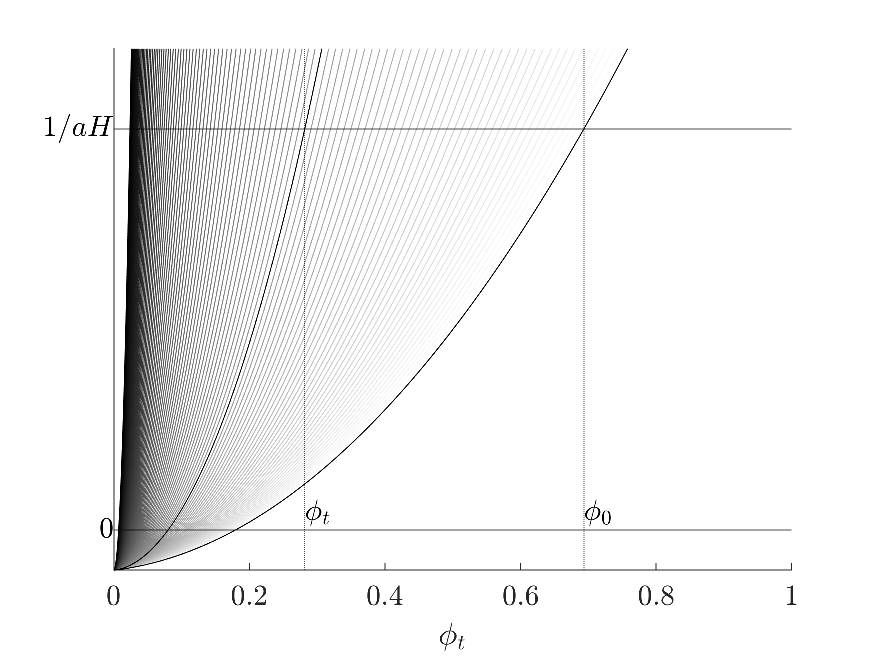
\includegraphics[width=0.7\linewidth]{fig_GH_phi.pdf}
    \caption{Determination of equilibrium $\phi_t$.}
    \label{fig:GH_phi}
    \caption*{\footnotesize Note: The numerical example is based on parameter values $\beta=1/2$, $\alpha=1/2$, $\rho=2$, $\theta=1/2$, $A_XH=10$, $A_LL=1$, $\xi_u=0.7$, $\lambda_u=0.2$, $\xi_b=\lambda_b=0.1$, $aH=0.2$, and $n_0=1$.}
\end{figure}

We are now ready to show the emergence of stochastic bubbles. Because agents have homogeneous preferences, we may use the SDF of type $H$ agents. Using the optimal consumption $c_{Ht}^y=(1-\beta)w_{Ht}$ and the indifference condition \eqref{eq:indifference}, we obtain
\begin{equation*}
    c_{Ht}^y=(1-\beta)Q_tan_t.
\end{equation*}
Using the old's budget constraint \eqref{eq:budget_GH_old} and asset demand \eqref{eq:nHt}, we obtain
\begin{equation*}
    c_{H,t+1}^o=\beta an_t(Q_{t+1}+D_{t+1}).
\end{equation*}
Substituting these two equations in the SDF \eqref{eq:SDF} and noting that $n_t$ is predetermined, we obtain the exact same SDF \eqref{eq:SDF_Q} as in \S\ref{sec:toy}. Therefore, the asset pricing implications are the same as the toy model in \S\ref{sec:toy} by identifying $(\beta e_t,D_t)\equiv (Q_t,D_t)$. Thus, to determine the existence or nonexistence of bubbles, it suffices to check the assumptions of Theorem \ref{thm:bubble_toy}.

Using \eqref{eq:divyield1} and \eqref{eq:laborH}, we obtain the dividend yield
\begin{equation}
    \frac{D_t}{Q_t}=aH\frac{1-\theta}{\theta}\phi_t. \label{eq:divyield2}
\end{equation}
Once state $b$ is reached, because $\phi_t$ is constant at $\phi_b$ in Proposition \ref{prop:growth}, Assumption \ref{asmp:balanced} holds and there are no bubbles by Proposition \ref{prop:nobubble_toy}: $Q_t=V_t$. Furthermore, the price-dividend ratio $Q_t/D_t$ is constant.

We next verify the assumptions of Theorem \ref{thm:bubble_toy}. Because uncertainty is driven only by the state $z_t\in \set{u,b}$, Assumption \ref{asmp:conditional} clearly holds. Conditional on staying in state $u$, since $\phi_t$ converges to 0 by Proposition \ref{prop:growth}, the price-dividend ratio $Q_t/D_t$ diverges to infinity. To show the existence of bubbles, it suffices to check the two conditions in \eqref{eq:finite_sum}. Following the notation in Theorem \ref{thm:bubble_toy}, let $x_t^z$ be the value of a variable $x_t$ conditional on $z_0=\dots=z_{t-1}=u$ and $z_t=z$. By \eqref{eq:n_dyn}, $n_t$ is determined at $t-1$, so we do not need the superscript $z$. Using $\phi_t\ge 0$ and $G_u\coloneqq 1+aH>1$, we obtain the trivial upper bound
\begin{equation}
    n_t\le n_0G_u^t \label{eq:nt_ub}
\end{equation}
from \eqref{eq:n_dyn}. By Proposition \ref{prop:growth}\ref{item:growth_u}, we have $\phi_t\to 0$ as $t\to\infty$. Therefore, for any $\epsilon>0$, we can take a constant $n_\epsilon>0$ such that the lower bound
\begin{equation}
    n_t \ge n_\epsilon (G_u-\epsilon)^t \label{eq:nt_lb}
\end{equation}
holds for all $t$. Let $\psi\coloneqq (\xi_u-\lambda_u)(\rho-1)>0$. Using $\phi_t>0$ in \eqref{eq:eqcond2}, we obtain
\begin{equation}
    \frac{1}{aH}\ge -1+\beta+\frac{\beta(1-\alpha)}{\theta\alpha}\left(\frac{A_XH}{A_LL}\right)^{\rho-1}n_t^\psi(\phi_t^u)^\rho \iff \phi_t^u\le C_\phi n_t^{-\psi/\rho} \label{eq:phit_ub}
\end{equation}
for some constant $C_\phi>0$ (because $1-\beta>0$). Since $G_u=1+aH>1$, we can choose $\epsilon>0$ such that $G_u-\epsilon>1$. Hence combining \eqref{eq:divyield2}, \eqref{eq:phit_ub}, and \eqref{eq:nt_lb}, we obtain
\begin{equation*}
    \frac{D_t^u}{Q_t^u}\le aH\frac{1-\theta}{\theta}C_\phi n_t^{-\psi/\rho}\sim (G_u-\epsilon)^{-(\psi/\rho)t},
\end{equation*}
so $\sum_{t=1}^\infty D_t^u/Q_t^u<\infty$ and \eqref{eq:finite_sum1} holds by identifying $(\beta e_t,D_t)\equiv (Q_t,D_t)$.

Using the output \eqref{eq:prod_Y}, the CES production function \eqref{eq:F_CES}, skilled labor input \eqref{eq:laborH}, and the productivities \eqref{eq:AXLt}, we obtain the output
\begin{equation}
    Y_t=\left[\alpha(A_Xn_t^{\xi_{z_t}}\phi_tH)^{1-\rho}+(1-\alpha) (A_Ln_t^{\lambda_{z_t}}L)^{1-\rho}\right]^\frac{1}{1-\rho}. \label{eq:Yt_CES}
\end{equation}
Conditional on $z_0=\dots=z_{t-1}=u$ and $z_t=b$, we have $n_t\sim G_u^t$ and $\phi_t=\phi_b$ (constant). Since $\lambda_b=\xi_b$ by Assumption \ref{asmp:AZ}, we obtain
\begin{equation}
    Y_t^b\sim n_t^{\lambda_b}\sim G_u^{\lambda_bt}. \label{eq:Yb_order}
\end{equation}
In state $u$, we have $n_t^{\lambda_{z_t}}=n_t^{\lambda_u}$ and $n_t^{\xi_{z_t}}\phi_t\sim n_t^{\xi_u-\psi/\rho}$ by \eqref{eq:phit_ub}. Using the definition of $\psi$, the exponents of $n_t$ inside the bracket of \eqref{eq:Yt_CES} are ordered according to
\begin{equation*}
    (1-\rho)(\xi_u-\psi/\rho)\gtrless (1-\rho)\lambda_u \iff -\rho\psi\gtrless (1-\rho)\psi \iff \psi \lessgtr 0.
\end{equation*}
Since $\psi>0$ by \eqref{eq:xi} and $n_t\sim G_u^t$, we have
\begin{equation}
    Y_t^u\sim n_t^{\lambda_u}\sim G_u^{\lambda_ut}. \label{eq:Yu_order}
\end{equation}
Using \eqref{eq:eqprice_Q}, the CES production function \eqref{eq:F_CES}, skilled labor input \eqref{eq:laborH}, and the productivities \eqref{eq:AXLt}, we obtain the stock price
\begin{equation*}
    Q_t=\frac{\theta}{an_t}\alpha Y_t^\rho A_{Xt}^{1-\rho}X_t^{-\rho}=\frac{\theta\alpha}{an_t}Y_t^\rho (A_Xn_t^{\xi_{z_t}})^{1-\rho}(\phi_t H)^{-\rho}.
\end{equation*}
Taking the ratio between states $b$ and $u$ and noting that $n_t$ is determined at $t-1$, we obtain
\begin{align}
    \frac{Q_t^b}{Q_t^u}&=(Y_t^b/Y_t^u)^\rho n_t^{(\xi_b-\xi_u)(1-\rho)}(\phi_b/\phi_t^u)^{-\rho} \notag \\
    &\sim n_t^{(\lambda_b-\lambda_u)\rho}n_t^{(\xi_b-\xi_u)(1-\rho)}n_t^{-\psi}=n_t^{\lambda_b-\lambda_u}, \label{eq:Q_ratio}
\end{align}
where we have used the order of magnitude \eqref{eq:Yb_order} and \eqref{eq:Yu_order}, the definition of $\psi$ in \eqref{eq:xi}, and $\lambda_b=\xi_b$ (condition \eqref{eq:alphazeta}). The same order of magnitude holds for $Q_t+D_t$ instead of $Q_t$ because
\begin{equation*}
    \frac{Q_t^b+D_t^b}{Q_t^u+D_t^u}=\frac{Q_t^b}{Q_t^u}\frac{1+D_t^b/Q_t^b}{1+D_t^u/Q_t^u},
\end{equation*}
$D_t^b/Q_t^b$ is constant using \eqref{eq:divyield2} and $\phi_t^b=\phi_b$, and $D_t^u/Q_t^u\to 0$. Since $\lambda_u>\lambda_b$ and $n_t\sim (G_u-\epsilon)^t$, it follows that \eqref{eq:finite_sum2} holds if $\gamma<1$. Consequently, we obtain the following theorem, which is our main result.

\begin{thm}\label{thm:bubble_GH}
Suppose the aggregate production function takes the CES form \eqref{eq:F_CES}, Assumptions \ref{asmp:utility}, \ref{asmp:states}, \ref{asmp:AZ}, \ref{asmp:n0} hold, and relative risk aversion is $\gamma<1$. Let $Q_t$ be the stock price in the unique equilibrium established in Proposition \ref{prop:eq_GH} and $V_t$ be its fundamental value. Then the following statements are true.
\begin{enumerate}
    \item In state $z_t=u$, the stock price exhibits a bubble: $Q_t>V_t$ and the price-dividend ratio $Q_t/D_t$ grows exponentially.
    \item In state $z_t=b$, the stock price reflects fundamentals: $Q_t=V_t$ and the price-dividend ratio $Q_t/D_t$ is constant.
\end{enumerate}
\end{thm}

In \S\ref{sec:toy}, we pointed out the conditions to generate a stochastic bubble are \ref{item:imp3a} during unbalanced growth, endowments (stock prices) grow faster than dividends, and \ref{item:imp3b} when the economy switches to balanced growth, endowments (stock prices) sufficiently decline. We can explain the correspondence as follows. Looking at the dividend yield formula \eqref{eq:divyield2} and the bound for $\phi_t$ in \eqref{eq:phit_ub}, it is clear that $\psi=(\xi_u-\lambda_u)(\rho-1)>0$ (condition \eqref{eq:xi}) ensures condition \ref{item:imp3a}: under this condition, the price-dividend ratio rises exponentially. Similarly, looking at \eqref{eq:Q_ratio}, $\lambda_u>\lambda_b=\xi_b$ (condition \eqref{eq:alphazeta}) ensures condition \ref{item:imp3b}: under this condition, upon switching to balanced growth, the relative stock price $Q_t^b/Q_t^u\sim n_t^{\lambda_u-\lambda_b}$ becomes smaller the longer state $u$ persists.

There are three messages to be drawn from Theorem \ref{thm:bubble_GH}. \begin{enumerate*}
    \item First, temporary unbalanced technological growth driven by regime switching together with some conditions on elasticities (\eg, elasticity of substitution between production factors, relative risk aversion, and relative strengths of spillover effects) necessarily generates stock market bubbles. 
    \item Second, the dynamics of the price-dividend ratio is markedly different depending on the aggregate state $z\in \set{u,b}$ \ie, before and after the collapse of the bubble economy. With the emergence of the stock price bubble, the price-dividend ratio initially rises exponentially and then decreases substantially with the collapse of the bubble economy. 
    \item Third, we learn that the dynamics with unbalanced growth and stock bubbles can be seen as a temporary deviation from the balanced growth path. Intuitively, when $\lambda_u>\lambda_b=\xi_b$, \ie, the spillover effects of innovation are high, and $\xi_u \neq \lambda_u$, then the positive effects of innovation are unevenly spread over the two production factors $A_{Xt}X_t$ and $A_{Lt}L$. This causes a divergence in their productivity growth rates, leading to unbalanced growth. If households' relative risk aversion is sufficiently low ($\gamma<1$), this unbalanced growth, in turn, leads to a stock price bubble in industries that drive innovation. In other words, households with high risk tolerance begin to trade stocks in innovation-driven industries for speculative resale purposes.
\end{enumerate*}

When $\rho>1$, \ie, the elasticity of substitution between the two production factors $1/\rho$ is less than one, since \eqref{eq:xi} requires $\xi_u>\lambda_u$, bubbles are attached to the price of intangible capital with higher growth rates. However, once the state $u$ with high spillover ends and the spillover effects of innovation are evenly spread across the two factors of production ($\lambda_u>\lambda_b=\xi_b$), the economy transitions to the balanced growth path, and the stock price bubble bursts. Our model suggests that stock bubbles emerge in the process of spillover of technological innovation, which is consistent with the narrative in \citet{Scheinkman2014}.

Two remarks are in order. \begin{enumerate*}
    \item First, economic agents expect that the exponential rise in the price-dividend ratio will eventually come to an end. Despite this, the stock bubble inevitably emerges with the arrival of innovation.
    \item Second, this dynamics of the theoretical price-dividend ratio has the potential to connect our analysis with the econometric literature \citep*{PhillipsShiYu2015,PhillipsShi2018,PhillipsShi2020}, which purports to detect bubbles by explosive dynamics in the price-dividend ratio.
\end{enumerate*}

Figure \ref{fig:GH_PD} shows the dynamics of the price-dividend ratio for the same numerical example as in Figure \ref{fig:GH_phi}, computed as the reciprocal of the dividend yield \eqref{eq:divyield2}. Here, we suppose that the state $u$ persists until $t=39$ but switches to $b$ at $t=40$. During the bubble, the price-dividend ratio grows exponentially. Once the bubble bursts, the price-dividend ratio becomes a constant (because $\phi_b$ is constant) and the economy switches to balanced growth.

\begin{figure}[htb!]
    \centering
    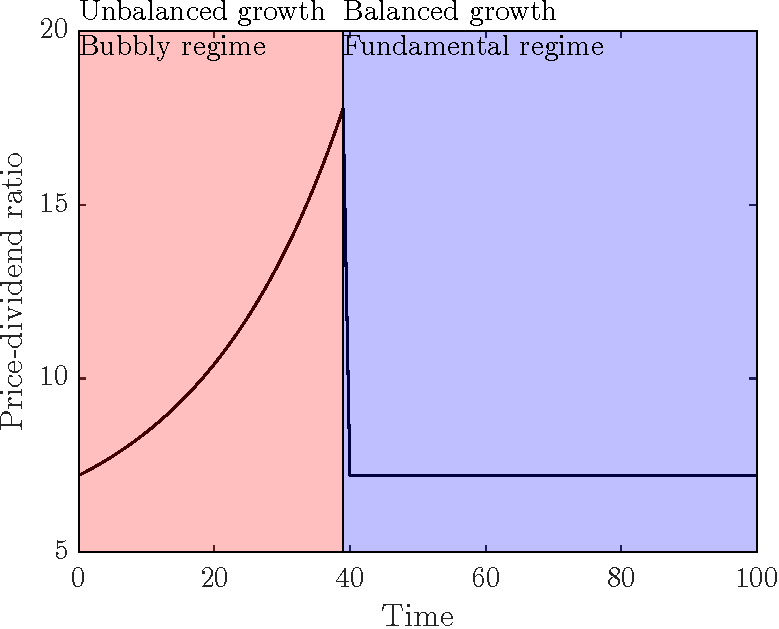
\includegraphics[width=0.7\linewidth]{fig_GH_PD.pdf}
    \caption{Dynamics of price-dividend ratio.}
    \label{fig:GH_PD}
\end{figure}

Although the relationship between rational bubbles and the divergence of the price-dividend ratio (see the remarks after Theorem \ref{thm:bubble_toy}) was likely not well known at the time, Kazuo Ueda, the current Governor of the Bank of Japan, seemed to have understood it intuitively more than three decades ago. \citet[p.~27]{Ueda1990} suggested the possibility of a stock price bubble starting in the mid-1980s, stating (translated from Japanese):

\begin{quote}
Japanese stock prices are abnormally high compared to real corporate performance such as earnings and dividends. [\ldots] If a stock price bubble occurs while corporate performance remains stagnant, dividend yields will converge to zero, and capital gains will account for most of the return on stock investments. In other words, recent stock price movements are consistent with the theory that they reflect a bubble.
\end{quote}

Indeed, when the dividend yield converges to zero, we can write the net stock return as
\begin{equation*}
    \frac{Q_t+D_t}{Q_{t-1}}-1=\underbrace{\frac{Q_t-Q_{t-1}}{Q_{t-1}}}_\text{capital gain}+\frac{Q_t}{Q_{t-1}}\times\underbrace{\frac{D_t}{Q_t}}_{\text{dividend yield}\approx 0},
\end{equation*}
so stock returns asymptotically consist solely of capital gains from speculative resale.

\subsection{Short- and long-term effects of stock bubbles}

Proposition \ref{prop:growth} shows that knowledge $n_t$ grows faster during the stock market bubble (state $u$). However, this effect confounds two causes, namely that
\begin{enumerate*}
    \item productivity growth is higher during state $u$ and
    \item there is a bubble during state $u$.
\end{enumerate*}
We now discuss the pure short- and long-term effects of the stock market bubble.

Suppose the economy is in state $u$. In the model, the skilled wage is determined by the indifference condition \eqref{eq:indifference} $an_tQ_t=w_{Ht}$. In a counterfactual economy without a stock market bubble, the stock price would be equal to the fundamental value $V_t<Q_t$, so the indifference condition would be $an_tV_t=w_{Ht}$. Noting that $n_t$ is determined at $t-1$, we derive the following observation.

\begin{obs}\label{obs:wH}
The stock market bubble tends to increase the skilled wage.
\end{obs}

By Proposition \ref{prop:eq_GH}, the skilled wage $w_{Ht}$ equals $\theta F_XA_{Xt}$, where the marginal product $F_X$ is evaluated at $(A_{Xt}H\phi_t,A_{Lt}L)$. Noting that the production function $F$ is concave and the productivities $A_{Xt},A_{Lt}$ are predetermined (because they are given by \eqref{eq:AXLt}, and $n_t$ is determined at time $t-1$), the increase in the skilled wage $w_{Ht}$ must be accompanied with a decrease in $\phi_t$, the fraction of skilled agents working in the knowledge-intensive good sector. In other words, the fraction of skilled agents engaging in R\&D must rise. Thus, we derive the following observation.

\begin{obs}\label{obs:innovation}
The stock market bubble tends to promote innovation.
\end{obs}

During the stock market bubble, high stock valuations and lucrative IPO profits incentivize skilled agents to innovate, which increases wages, which increases the demand for stocks and sends their prices even higher. This positive feedback loop creates a virtuous cycle of rising stock prices and innovation.

Again, by Proposition \ref{prop:eq_GH}, the unskilled wage $w_{Lt}$ equals $\theta F_LA_{Lt}$ evaluated at $(A_{Xt}H\phi_t,A_{Lt}L)$. As the stock market bubble decreases $\phi_t$, unskilled labor $L$ becomes relatively more abundant, which suppresses its wage. Thus, we derive the following observation.

\begin{obs}\label{obs:wL}
The stock market bubble tends to increase the wage gap between skilled and unskilled agents.
\end{obs}

This observation is at least consistent with \citet[Figure 18]{JovanovicRousseau2005} and \citet[\S4]{VanReenen2011}, which show that the wage gap increased with the arrival of the IT wave.

Now, suppose that the state transitions to $b$ at time $t$ and the bubble bursts. Noting that $\lambda_b=\xi_b$ and the production function is homogeneous of degree 1, the output \eqref{eq:prod_Y} is
\begin{equation}
    Y_t=F(A_XH\phi_b,A_LL)n_t^{\lambda_b}. \label{eq:Ytb}
\end{equation}
In contrast, using $\psi>0$, the output before the bubble bursts has an order of magnitude
\begin{equation}
    Y_{t-1}=F(A_{X,t-1}H\phi_t,A_{L,t-1}L)\sim (1-\alpha)^\frac{1}{1-\rho}A_LLn_{t-1}^{\lambda_u}. \label{eq:Yt-1}
\end{equation}
Dividing \eqref{eq:Ytb} by \eqref{eq:Yt-1} and noting that $n_t/n_{t-1}\sim 1+aH$, upon the collapse of the bubble, output grows by the factor
\begin{equation*}
    \frac{Y_t}{Y_{t-1}}\sim \frac{F(A_XH\phi_b,A_LL)(1+aH)^{\lambda_u}}{(1-\alpha)^\frac{1}{1-\rho}A_LL}n_t^{\lambda_b-\lambda_u}.
\end{equation*}
Since $\lambda_u>\lambda_b$, the larger $n_t$, the more severe the economic contraction is. Recall that $n_t$ grows over time according to \eqref{eq:n_dyn}, and the growth rate is higher if there is more innovation ($1-\phi_t$ is larger). Thus, combined with Observation \ref{obs:innovation}, we derive the following observation.

\begin{obs}\label{obs:contract}
The longer the stock market bubble lasts, the more severe the economic contraction when it bursts.
\end{obs}

Finally, we discuss long-term effects. In the long run, the state of the economy switches to $b$ and the stock market bubble collapses. The output is given by \eqref{eq:Ytb}, which depends on time only through knowledge $n_t$. By the same reasoning, we derive the following observation.

\begin{obs}\label{obs:output}
The stock market bubble tends to increase the output in the long run.
\end{obs}

This observation gives us an important insight into the bright side of temporary stock price bubbles. During the bubble period, the economy enjoys the innovation of a wide variety of goods and technologies. Even after the bubble collapses, the technologies developed during the bubble period survive, resulting in a permanently higher output level even after the collapse. To illustrate this point, Figure \ref{fig:GH_Y} plots the dynamic paths of output \eqref{eq:Yt_CES}, where in one case the bubble is short (bursting at $t=30$) and in the other case it lasts longer (bursting at $t=50$). After the collapse of the bubble, the economy returns to balanced growth with a growth rate independent of the history (Proposition \ref{prop:growth}\ref{item:growth_b}). However, because new technologies accumulate during the bubble period, the longer the bubble, the higher the level of the output. This figure implies that the stock bubble benefits not only the pre-bubble-burst generations but also the post-bubble-burst generations. As noted in the introduction, this bright side of stock bubbles is also consistent with the narrative highlighted by \citet{Scheinkman2014}, \ie, stock bubbles may have positive effects on innovative investments and economic growth.

\begin{figure}[htb!]
    \centering
    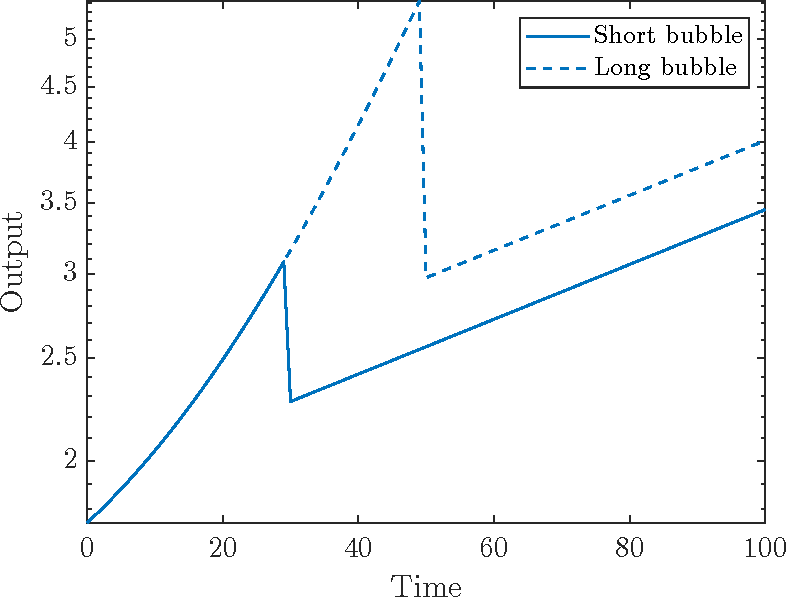
\includegraphics[width=0.7\linewidth]{fig_GH_Y.pdf}
    \caption{Dynamics of output.}
    \label{fig:GH_Y}
\end{figure}

The implications for wages are similar. Because $F$ is homogeneous of degree 1, the marginal products $F_X,F_L$ are homogeneous of degree 0. Hence by Proposition \ref{prop:eq_GH}, wages in state $b$ are given by
\begin{align*}
    w_{Ht}&=\theta F_X(A_XH\phi_b,A_LL)A_Xn_t^{\lambda_b}, \\
    w_{Lt}&=F_L(A_XH\phi_b,A_LL)A_Ln_t^{\lambda_b},
\end{align*}
which also depend on time only through knowledge $n_t$. Furthermore, the wage ratio $w_{Lt}/w_{Ht}$ is constant. Thus, we derive the following observation.

\begin{obs}\label{obs:wage}
The stock market bubble tends to increase wages in the long run but does not affect the wage gap between skilled and unskilled agents.
\end{obs}

This observation captures another bright aspect of stock bubbles that the stock bubble not only has a positive effect on wages of the generation that experienced the bubble economy, but also increases overall wages of the post-bubble generation, because the technologies created during the bubble period will remain.

\subsection{Implication for macro-financial modeling}\label{sec:uzawa}

Our Theorem \ref{thm:bubble_GH} implies that, under some conditions on elasticities (\eg, elasticity of substitution between production factors, relative risk aversion, and relative strengths of spillover effects), stock market bubbles that are expected to burst emerge as the unique equilibrium outcome and that the price-dividend ratio will rise exponentially as long as the bubble persists. Readers may be skeptical that the assumptions are special. The following proposition shows that ruling out bubbles requires even more special (knife-edge) assumptions.

\begin{prop}\label{prop:knife-edge}
Let everything be as in the general model of \S\ref{subsec:innovation_model}, where we only impose Assumptions \ref{asmp:utility} and \ref{asmp:F}. If there is innovation ($\phi_t<1$), the price-dividend ratio $Q_t/D_t$ is constant over time if and only if either the relative productivity $A_{Xt}/A_{Lt}$ is constant or the production function $F$ is Cobb-Douglas. In particular, in the setting of Theorem \ref{thm:bubble_GH}, the parameters need to satisfy
\begin{equation}
    \psi=(\xi_u-\lambda_u)(\rho-1)=0. \label{eq:knife-edge}
\end{equation}
\end{prop}

Note that Proposition \ref{prop:knife-edge} requires only the neoclassical production function, so it is independent of the special features assumed in Theorem \ref{thm:bubble_GH}. Proposition \ref{prop:knife-edge} somehow resembles the Uzawa steady-state growth theorem, which is at the heart of macro-growth theory. \citet[p.~118]{Uzawa1961} defined a time-varying neoclassical production function $F(K,L,t)$ to be Harrod-neutral if the marginal product of capital $F_K(K,L,t)$ (\ie, interest rate) is constant if the capital-output ratio $K/F(K,L,t)$ is constant. \citet{Uzawa1961} proved that 
\begin{enumerate*}
    \item $F$ is Harrod-neutral if and only if $F(K,L,t)$ takes the form $F(K,A(t)L)$, \ie, technical change is only labor-augmenting and that
    \item with such a specification, a balanced growth path in which capital and output grow at the same rate exists.
\end{enumerate*}

Subsequently, the Uzawa steady-state growth theorem came to mean that if a neoclassical growth model exhibits balanced growth, then technical change must be labor-augmenting \citep{JonesScrimgeour2008}. \citet{Schlicht2006} proved a variant of this result that if output, capital, and consumption all grow exponentially (at potentially different but constant rates), then the production function must take the form $F(K,A(t)L)$ where labor-augmenting productivity $A(t)$ grows exponentially. Ruling out capital-augmenting productivity growth is a knife-edge restriction. If the production function is Cobb-Douglas, then $F(A_KK,A_LL)=(A_KK)^\alpha(A_LL)^{1-\alpha}=K^\alpha (AL)^{1-\alpha}$ with $A\coloneqq A_K^\frac{\alpha}{1-\alpha}A_L$, so we may always reinterpret any factor-augmenting productivities as purely labor-augmenting. However, the Cobb-Douglas production function itself is a knife-edge restriction.

The fact that some knife-edge restriction is necessary for obtaining a balanced growth path is a common feature of all growth models. \citet[\S15.6]{Acemoglu2009} constructs a model of directed technological change, where the productivity growth of two production factors is determined by two sectors of R\&D investment. He shows that balanced growth can only be achieved under a knife-edge condition.
\citet*{GrossmanHelpmanOberfieldSampson2017} consider a general neoclassical production function and obtain balanced growth, despite the presence of capital-augmenting technological progress. Nevertheless, they still require knife-edge conditions, noting ``As with any model that generates balanced growth, knife-edge restrictions are required to maintain the balance; our model is no exception to this rule'' (p.~1306).

Returning to Proposition \ref{prop:knife-edge}, what it implies is that to obtain a stable price-dividend ratio, the production function or factor-augmenting productivities must satisfy some knife-edge restrictions. We conjecture that this is true in any production-based asset pricing model. This observation has an important implication for macro-financial modeling. In many models, it seems that stability in dividend-output ratio is imposed either outright by considering a consumption-based asset pricing model with balanced consumption and dividends or by a production-based asset pricing model with special features. Such models will feature balanced growth and can never generate bubbles by model construction. However, once we move away from knife-edge restrictions, allowing unbalanced growth, even if only temporarily, asset price bubbles naturally arise.

\section{Concluding remarks}\label{sec:conclusion}

As noted in the introduction, any balanced growth model is knife-edge theory. By imposing knife-edge restrictions, macro-finance models that generate only a BGP, including a single dynamic path converging to it, are constructed from the outset so that asset prices reflect fundamentals. We have shown that the slightest deviation from knife-edge cases leads to markedly different asset pricing implications. To illustrate this point, as an example of a full-fledged macro-finance model, we have employed the variety expansion model of \citet[Ch.~3]{GrossmanHelpman1991book}. Our approach that allows for the possibility of unbalanced growth and considers regime switching between unbalanced growth and balanced growth can generally be applied to other innovation-driven growth models, including \citet{Romer1990}, \citet{GrossmanHelpman1991}, and \citet{AghionHowitt1992}. 

Similarly, in many cases, by imposing knife-edge conditions, macro-finance models are constructed from the outset so that the economy converges to a steady state characterized by balanced growth. In other words, the economy is always on the same dynamic path, which usually corresponds to a saddle path that can be drawn with one stroke of the brush. By adding various types of exogenous shocks or by changing the magnitude of those shocks, macro-finance models have attempted to account for fluctuations in asset prices qualitatively and quantitatively, which has produced fruitful outcomes up to present. In light of this existing approach, it would be fair to say that our methodology of macro-financial modeling would provide a different approach. That is, our approach of removing the knife-edge restrictions allows the economy to temporarily take a different dynamic path from a balanced growth path or a single dynamic path converging to it. As our paper has illustrated, this deviation from the BGP would result in markedly different implications for asset pricing. In other words, the dynamic path with asset price bubbles can be understood as a temporary deviation from the BGP.

\appendix

\section{Proofs}\label{sec:proof}

\subsection{Proof of Proposition \ref{prop:nobubble_b}}

Without loss of generality, assume $z_0=b$. Because uncertainty is resolved, the stochastic discount factor \eqref{eq:SDF_Q} reduces to $m_{t\to t+1}=Q_t/(Q_{t+1}+D_{t+1})$. Therefore,
\begin{equation}
    m_{0\to t}Q_t=\frac{Q_0}{Q_1+D_1}\times\dots\times \frac{Q_{t-1}}{Q_t+D_t}\times Q_t=Q_0\prod_{s=1}^t\frac{Q_s}{Q_s+D_s}. \label{eq:mQ_b}
\end{equation}
By Assumption \ref{asmp:balanced}, $D_t/e_t=D_{t+1}/e_{t+1}$ is constant (that may depend on history). Since $Q_t=\beta e_t$ by Proposition \ref{prop:eq_toy}, the dividend yield $D_t/Q_t$ is also constant, so $\frac{Q_s}{Q_s+D_s}=\frac{1}{1+D_s/Q_s}$ is a positive constant less than 1. Therefore $\lim_{t\to\infty}\E_0[m_{0\to t}Q_t]=0$ and the no-bubble condition \eqref{eq:nobubble} holds. \hfill \qedsymbol

\subsection{Proof of Proposition \ref{prop:nobubble_toy}}



Fix $j\in \N$ and suppose $\tau=j$. For $t>j$, it follows from the same derivation as \eqref{eq:mQ_b} that
\begin{align}
    m_{0\to t}Q_t&=m_{0\to j}\frac{Q_j}{Q_{j+1}+D_{j+1}}\times \dots \times \frac{Q_{t-1}}{Q_t+D_t}\times Q_t \notag \\
    &=m_{0\to j}Q_j\prod_{s=j+1}^t\frac{Q_s}{Q_s+D_s}. \label{eq:mQ_j}
\end{align}
For $s>j$, by Assumption \ref{asmp:balanced} and $Q_t=\beta e_t$, the ratio $\frac{Q_s}{Q_s+D_s}=\frac{1}{1+D_s/Q_s}$ is a positive constant (depending on history) less than 1. Therefore, \eqref{eq:mQ_j} converges to 0 almost surely as $t\to \infty$. Furthermore, it is bounded by $m_{0\to j}Q_j$, which is integrable because \eqref{eq:Q_iter} implies $\E_0[m_{0\to j}Q_j]\le Q_0$. By the dominated convergence theorem, we obtain
\begin{equation*}
    E_{jt}\coloneqq \E_0[m_{0\to t}Q_t \mid \tau=j]\to 0
\end{equation*}
as $t\to\infty$, and convergence is monotone because the right-hand side of \eqref{eq:mQ_j} is decreasing in $t$. Let $\mu$ be the probability measure on $\N=\set{1,2,\dotsc}$ defined by $\mu(j)=\pi^{j-1}(1-\pi)$. Then by definition, we have
\begin{equation*}
    \sum_{j=1}^t\pi^{j-1}(1-\pi)\E_0[m_{0\to t}Q_t \mid \tau=j]=\int_{\N} E_{jt}\diff \mu(j),
\end{equation*}
where we define $E_{jt}=0$ for $j>t$. Since $E_{jt}\downarrow 0$ as $t\to \infty$, by the monotone convergence theorem, we obtain
\begin{equation*}
    \lim_{t\to\infty}\sum_{j=1}^t\pi^{j-1}(1-\pi)\E_0[m_{0\to t}Q_t \mid \tau=j]=0.
\end{equation*}
By \eqref{eq:mQ_iter}, we have $\E_0[m_{0\to t}Q_t]\to 0$ if and only if \eqref{eq:TVC} holds. 

If $(e_t,D_t)$ is $\F_{t-1}$-measurable or $\gamma=1$, the stochastic discount factor \eqref{eq:SDF} becomes $m_{t\to t+1}=Q_t/(Q_{t+1}+D_{t+1})$. Then \eqref{eq:mQ_b} remains valid, and we have $m_{0\to t}Q_t\le Q_0$. The last term in \eqref{eq:mQ_iter} can be bounded above as
\begin{equation*}
    \pi^t\E_0[m_{0\to t}Q_t \mid \tau>t]\le \pi^t Q_0\to 0
\end{equation*}
as $t\to \infty$, so \eqref{eq:TVC} holds and there is no bubble. \hfill \qedsymbol

\subsection{Proof of Proposition \ref{prop:eq_GH}}

We first derive the equilibrium condition \eqref{eq:eqcond1}. Suppose an equilibrium with $\phi_t>0$ exists. Given $\phi_t$, the knowledge-intensive good $X_t$ is uniquely determined by \eqref{eq:laborH}. Then the output $Y_t$ is determined by \eqref{eq:prod_Y}, which determines $w_{Lt}$ and $P_t=p_t(j)$ by \eqref{eq:wLt} and \eqref{eq:Pt}. Using \eqref{eq:ptj}, we obtain $w_{Ht}=\theta P_t$. Thus combining \eqref{eq:nHLt}, \eqref{eq:n_dyn}, and \eqref{eq:n_clear}, we obtain the equilibrium condition
\begin{equation*}
    (1+a(1-\phi_t)H)n_t=H\beta an_t+L\frac{F_LA_{Lt}}{\theta F_XA_{Xt}}\beta an_t,
\end{equation*}
where $F_X,F_L$ are evaluated at $(A_{Xt}X_t,A_{Lt}L)=(A_{Xt}\phi_t H,A_{Lt}L)$. Dividing both sides by $an_tH>0$ and using the homogeneity of $F$ and the definition of $g$, we obtain
\begin{equation*}
    \frac{1}{aH}+1-\phi_t=\beta+\beta\left[\theta\frac{A_{Xt}H}{A_{Lt}L}g\left(\frac{A_{Xt}\phi_t H}{A_{Lt}L}\right)\right]^{-1},
\end{equation*}
which is equivalent to \eqref{eq:eqcond1}.

We next show the existence and uniqueness of equilibrium. Since $F$ is concave, $g(x)$ in Assumption \ref{asmp:F} is decreasing and has range $(0,\infty)$. Therefore, the right-hand side of \eqref{eq:eqcond1} is strictly increasing in $\phi_t$ and achieves a minimum of $\beta-1<0$ at $\phi_t=0$. Hence $\phi_t>0$ satisfying \eqref{eq:eqcond1} uniquely exists if and only if the right-hand side evaluated at $\phi_t=1$ exceeds the left-hand side, $1/(aH)$, which is precisely the condition \eqref{eq:phi_cond}. Since the equilibrium condition \eqref{eq:eqcond1} depends on $t$ only through $A_{Xt}/A_{Lt}$, so does $\phi_t$. If \eqref{eq:phi_cond} fails, then we can construct a unique equilibrium by setting $\phi_t=1$ and determining the stock price $Q_t$ by letting the market capitalization $Q_tn_{t+1}=Q_tn_t$ (because $1-\phi_t=0$) equal to aggregate savings $\beta (Hw_{Ht}+Lw_{Lt})$.

Finally, we prove \eqref{eq:eqprice}. \eqref{eq:eqprice_wL} and \eqref{eq:eqprice_P} follow from \eqref{eq:wLt} and \eqref{eq:Pt}. \eqref{eq:eqprice_wH} follows from $P_t=p_t(j)$ and \eqref{eq:ptj}. \eqref{eq:eqprice_Q} follows from the indifference condition $anQ_t=w_{Ht}$. \hfill \qedsymbol

\subsection{Proof of Proposition \ref{prop:growth}}

In state $u$, the equilibrium condition \eqref{eq:eqcond2} reduces to
\begin{equation}
    \frac{1}{aH}=\phi_t-1+\beta+\frac{\beta(1-\alpha)}{\theta\alpha}\left(\frac{A_XH}{A_LL}\right)^{\rho-1}n_t^{(\xi_u-\lambda_u)(\rho-1)}\phi_t^\rho. \label{eq:phiu_cond}
\end{equation}
At $t=0$, by Assumption \ref{asmp:n0}, there exists a unique $\phi_0\in (0,1)$ solving \eqref{eq:phiu_cond}. By \eqref{eq:n_dyn}, we have $n_{t+1}>n_t$, so knowledge monotonically increases. By condition \eqref{eq:xi}, fixing $\phi_t$, the right-hand side of \eqref{eq:phiu_cond} is strictly increasing in $t$. Therefore a unique solution $\phi_t\in (0,1)$ exists, which is strictly decreasing in $t$. Using \eqref{eq:n_dyn}, the growth rate of $n_t$ is bounded below by $1+a(1-\phi_0)H>1$. Therefore, $\set{n_t}$ diverges to infinity. Letting $t\to\infty$ in \eqref{eq:phiu_cond} and using \eqref{eq:xi}, we must have $\phi_t\to 0$. Again using \eqref{eq:n_dyn}, $n_t$ asymptotically grows at rate $G_u\coloneqq 1+aH$.

In state $b$, the equilibrium condition \eqref{eq:eqcond2} reduces to \eqref{eq:phib_cond2}. Such $\phi_b\in (0,1]$ exists if and only if \eqref{eq:phib_cond1} holds. Otherwise, we have $\phi_b=0$ by Proposition \ref{prop:eq_GH}. Using \eqref{eq:n_dyn}, $n_t$ grows at rate $G_b\coloneqq 1+a(1-\phi_b)H$. \hfill \qedsymbol

\subsection{Proof of Proposition \ref{prop:knife-edge}}

If the price-dividend ratio $Q_t/D_t$ is constant, so is the dividend yield $D_t/Q_t$. Then \eqref{eq:divyield2} implies that $\phi_t$ is constant. Let this value be $\phi$. By assumption, $\phi<1$, so the equilibrium condition \eqref{eq:eqcond1} implies
\begin{equation*}
    \frac{1}{aH}=\phi-1+\beta+\beta\left[\theta\frac{A_{Xt}H}{A_{Lt}L}g\left(\frac{A_{Xt}H}{A_{Lt}L}\phi\right)\right]^{-1}.
\end{equation*}
Setting $x_t\coloneqq (A_{Xt}H/A_{Lt}L)\phi$ and rearranging terms yields
\begin{equation*}
    \frac{1}{\phi}\left(\frac{1}{aH}+1-\beta\right)=1+\frac{\beta}{\theta x_tg(x_t)}.
\end{equation*}
Therefore, $x_tg(x_t)$ is constant. If $x_t$ is constant, so is $A_{Xt}/A_{Lt}=(L/H)(x_t/\phi)$. If $A_{Xt}/A_{Lt}$ is not constant, then the function $x\mapsto xg(x)$ must be constant. Let $f(x)\coloneqq F(x,1)$. Using the homogeneity of $F$, we obtain $F_X(x,1)=f'(x)$ and $F_L(x,1)=f(x)-xf'(x)$. Therefore
\begin{equation*}
    xg(x)=x\frac{F_X(x,1)}{F_L(x,1)}=\frac{xf'(x)}{f(x)-xf'(x)}=c
\end{equation*}
for some $c>0$. Separating variables, we obtain
\begin{equation*}
    \frac{f'(x)}{f(x)}=\frac{c}{(1+c)x}\eqqcolon \frac{\alpha}{x},
\end{equation*}
where $\alpha\in (0,1)$. Since $(f(x)x^{-\alpha})'=f'(x)x^{-\alpha}-f(x)\alpha x^{-\alpha-1}=0$, the function $f(x)x^{-\alpha}$ must be constant and $f(x)=Ax^\alpha$ for some $A>0$. Therefore, $F(X,L)=Lf(X/L)=AX^\alpha L^{1-\alpha}$ is Cobb-Douglas.

Conversely, if $F$ is Cobb-Douglas, so $f(x)=Ax^\alpha$, then $xg(x)=\alpha/(1-\alpha)$ is constant and the equilibrium condition \eqref{eq:eqcond1} does not depend on time. The same holds if $A_{Xt}/A_{Lt}$ is constant, so $\phi_t$ is constant. \hfill \qedsymbol

\printbibliography

\end{document}